% ============================================================
%  findings.tex  —  Findings Section (Overleaf-compatible)
%  Stochastic Bellhop UQ: Delta Method, MC, PCE, LN3
% ============================================================
\documentclass[11pt,a4paper]{article}

\usepackage[margin=2.5cm]{geometry}
\usepackage{amsmath,amssymb}
\usepackage{graphicx}
\usepackage{booktabs}
\usepackage{multirow}
\usepackage{caption}
\usepackage{subcaption}
\usepackage{xcolor}
\usepackage{hyperref}
\usepackage{float}
\usepackage{tikz}
\usetikzlibrary{arrows.meta,decorations.pathreplacing,shapes.geometric}

% Figure path — set to figures subfolder or adjust per upload
\graphicspath{
  {Methods/MC/}
  {Methods/Delta/}
  {Methods/LN3/}
  {Methods/PCE/}
  {Methods/Comparison/}
  {validation/analytical/figures/}
}

\newcommand{\EX}{\mathbb{E}}
\newcommand{\Var}{\mathrm{Var}}
\newcommand{\TL}{\mathrm{TL}}
\newcommand{\Pshadow}{P_{\mathrm{shadow}}}

% ============================================================
\begin{document}
% ============================================================

% ────────────────────────────────────────────────────────────
\section*{Executive Summary}
\addcontentsline{toc}{section}{Executive Summary}

This report evaluates four uncertainty quantification (UQ) methods for
underwater acoustic transmission loss (TL) computed by the Bellhop ray-tracing
model.
The uncertain inputs are carrier frequency, source depth ($z_S$), and sound
velocity profile (SVP), each modelled as an independent random variable.
Three analytical methods --- the 2\textsuperscript{nd}-order Delta method,
Polynomial Chaos Expansion (PCE), and a 3-parameter lognormal (LN3) fit --- are
compared against Monte Carlo (MC) ground truth across five propagation scenarios
(baseline flat 50\,m, flat shallow 50\,m, flat deep 2500\,m, upslope, downslope)
and three input uncertainty distributions (Normal\,1/5/10\%).

\textbf{Key conclusions:}
\begin{itemize}
  \item The \textbf{Delta method} (1\textsuperscript{st}-order Taylor) is
        reliable for flat bathymetry and small perturbations ($\leq$1\%), but the
        2\textsuperscript{nd}-order Hessian correction already exceeds 96\% of the
        total variance at 5\% uncertainty, indicating the Taylor series has not
        converged.  Delta fails at slope bathymetry regardless of perturbation
        level.
  \item \textbf{PCE} (fitted to the existing $N=50$ MC samples at zero extra
        Bellhop cost) achieves $L_1 < 10\%$ convergence at order $K^* = 3$--$6$
        for deep-water SVP and frequency uncertainty, consistent with the
        published literature.  Source depth ($z_S$) resists polynomial convergence
        at all orders $K \leq 10$ in deep water --- a new finding not reported
        elsewhere.  Slope scenarios also require full MC.
  \item The \textbf{Delta--LN3 hybrid} (moment-matched shadow probability)
        performs well for flat scenarios but degrades at shadow-zone boundaries in
        slope environments.
  \item \textbf{Full Monte Carlo} is unavoidable for slope bathymetry ($\geq$5\%
        perturbation) and for $z_S$ in deep water with Normal distributions.
  \item The \textbf{LN3 distribution fit} (method of moments) is statistically
        suboptimal: MLE would be more efficient, but the LHS samples used throughout
        this pipeline are \emph{not} i.i.d.\ (stratification breaks independence),
        so the standard MLE log-likelihood is misspecified.  A design-weighted
        pseudo-likelihood or survey-sampling correction would be required for a
        rigorous MLE fit; this remains an open methodological limitation.
\end{itemize}

\textbf{Practical recommendation:} For sonar mission planning, use
PCE-$K^*$ (order 3--6) on flat-bottom scenarios and fall back to MC for slope
environments or large source-depth uncertainty.  Report $P_\mathrm{fail}$ and
P95 TL maps rather than variance alone, as variance does not distinguish the
\emph{direction} of acoustic uncertainty.

% ============================================================
\section{Results}

\subsection{Monte Carlo Reference Statistics}
\label{sec:mc}

Monte Carlo (MC) simulations with $N=1000$ samples per scenario and
distribution provide the reference statistics $\EX[\TL]$ and $\Var[\TL]$ against which
all analytical approximations are evaluated.
The sample pool combines Latin Hypercube (LHS), IID, and SVP-perturbed draws.
Figure~\ref{fig:mc_ex_var} shows representative $\EX[\TL]$ and $\Var[\TL]$ maps for
the five propagation scenarios under 5\% uniform source-depth ($z_S$) uncertainty.

\begin{figure}[H]
  \centering
  \begin{subfigure}[t]{0.48\textwidth}
    
\includegraphics[width=\linewidth]{shallow_water/Normal_5pct/figures/TL_zS.png}
    \caption{Shallow water (flat, 50\,m)}
  \end{subfigure}\hfill
  \begin{subfigure}[t]{0.48\textwidth}
    
\includegraphics[width=\linewidth]{deep_water/Normal_5pct/figures/TL_zS.png}
    \caption{Deep water (flat, 2500\,m)}
  \end{subfigure}\\[8pt]
  \begin{subfigure}[t]{0.48\textwidth}
    
\includegraphics[width=\linewidth]{downslope/Normal_5pct/figures/TL_zS.png}
    \caption{Downslope (50\,$\to$\,550\,m)}
  \end{subfigure}
  \caption{MC mean transmission loss $\EX[\TL]$ (dB re\,1\,$\mu$Pa) for Normal\,5\%
           $z_S$ perturbation across three representative scenarios.
           Colour scale: blue (low TL, strong signal) to red (high TL, shadow zone).
           The downslope scenario shows a marked refraction shadow at mid-range
           driven by the shoaling bathymetry.}
  \label{fig:mc_ex_var}
\end{figure}

\subsubsection{Input Sound-Velocity Profiles}
\label{sec:svp_ensemble}

Figure~\ref{fig:svp_ensemble} shows the $N=1000$ sampled SVP realisations for the
deep-water scenario under Normal\,5\% uncertainty.
Each blue trace is one Monte Carlo draw; the bold black curve is the nominal
summer-season profile.
The ensemble illustrates the physical spread driving acoustic variability:
a $\pm5\%$ perturbation in surface temperature shifts the mixed-layer depth by
$\pm$\,15\,m and changes the sound-speed gradient throughout the water column.

\begin{figure}[H]
  \centering
  
\includegraphics[width=0.45\linewidth]{deep_water/Normal_5pct/figures/svp_ensemble.png}
  \caption{SVP ensemble for deep-water scenario, Normal\,5\% uncertainty, $N=1000$.
           Blue traces: sampled profiles; black: nominal profile.
           Surface-temperature perturbations shift the mixed-layer depth and alter
           the sub-thermocline gradient, producing the spread in TL shown in
           Figure~\ref{fig:mc_ex_var}.}
  \label{fig:svp_ensemble}
\end{figure}

\subsubsection{MC Estimator Convergence}
\label{sec:mc_conv}

For a scalar random variable $Y$ with finite variance, the sample mean
$\bar Y_N$ converges to $\mu_Y$ at the classical CLT rate
$\mathrm{RMSE}(\bar Y_N) = \sigma_Y / \sqrt{N}$.
The sample variance $S_N^2$ converges at the same asymptotic rate but with a
larger prefactor: for a Gaussian parent,
\begin{equation}
  \mathrm{Var}(S_N^2) \;=\; \frac{2\sigma_Y^4}{N-1},
  \label{eq:var_of_var}
\end{equation}
so the relative error of $S_N^2$ is $\sqrt{2/(N-1)}\,/\,C_V^2$, where
$C_V = \sigma_Y/\mu_Y$ is the coefficient of variation.
In practice this means that a variance estimate requires roughly $2\times$ as
many samples as a mean estimate to reach the same relative error -- or
equivalently $\approx 4\times$ as many samples to match the absolute RMSE of
the mean.
The pipeline uses $N=300$ Latin-Hypercube samples drawn from the broadest
distribution (\textsc{Normal\,10\%}) and reweights via importance sampling (IS)
to obtain estimates for the narrower \textsc{Normal\,5\%} and
\textsc{Normal\,1\%} distributions.
IS reduces the effective sample size (Kish ESS $< N$) for narrower targets,
but the relative statistical gain outweighs the IS variance penalty because
the IS weights for Normal\,5\% and Normal\,1\% are moderate
($\text{ESS}/N \gtrsim 0.5$ in all scenarios).
The convergence of pixel-wise $\EX[\TL]$ and $\Var[\TL]$ as a function of
sub-sample size $N' \in \{10,20,30,50,75,100,150,200,300\}$ is documented in
\texttt{Methods/MC\_convergence/} and confirms that $N=300$ is sufficient for
the Var estimator to reach the $\lesssim 5\%$ relative RMSE target at the
10\% uncertainty level.

% ────────────────────────────────────────────────────────────
\subsection{First-Order Delta Method: Accuracy and Failure Modes}
\label{sec:delta}

\paragraph{Terminology note.}
The term \emph{Delta method} here refers to linearisation via perturbation calculus
(first-order Taylor expansion of the model output around the nominal parameter vector),
and should not be confused with the Dirac delta function or with finite-difference
approximations.
The same technique appears under different names in other fields:
\emph{FOSM} (First-Order Second-Moment method) in structural reliability and engineering,
\emph{GUM linearisation} in metrology \cite{bipm2008gum}, and
\emph{error propagation} in experimental physics textbooks.
In a statistics context ``Delta method'' is standard and unambiguous;
in an acoustics or engineering context the FOSM alias may help readers
avoid confusion.

The 1\textsuperscript{st}-order Delta method approximates variance as:
\begin{equation}
  \Var_1[\TL] \;\approx\; \sum_{i} J_i^2 \,\sigma_i^2,
  \qquad
  J_i = \frac{\partial \TL}{\partial \theta_i}\bigg|_{\boldsymbol{\theta}_0}
  \label{eq:delta1}
\end{equation}
where Jacobians $J_i$ are computed via central finite differences.
The 2\textsuperscript{nd}-order extension adds Hessian correction terms
$\tfrac{1}{2} H_{ii}^2 \kappa_i$ where $\kappa_i = \EX[\delta\theta_i^4]/\sigma_i^4 - 1$
is the excess kurtosis.

\subsubsection{Where Delta Performs Well}

For the \textbf{shallow-water} and \textbf{deep-water} scenarios under small perturbations
($\leq$1\% uncertainty), the Delta method achieves relative $L_1$ errors below
10\% in the variance maps (see Table~\ref{tab:analytical_l1} for the exact
per-distribution breakdown from the analytical waveguide validation).
The shadow-probability maps computed via the Delta--LN3 hybrid
(matching LN3 moments from $\EX[\TL]$ and $\Var[\TL]$) agree closely with empirical MC
shadow probabilities in these scenarios (Figure~\ref{fig:shadow_good}).

\begin{figure}[H]
  \centering
  % --- Row 1: flat scenario where Delta works (baseline, Uniform 1%) ---
  \begin{subfigure}[t]{0.48\textwidth}
    
\includegraphics[width=\linewidth]{shallow_water/Normal_1pct/figures/shadow_70_MC_vs_Delta_zS.png}
    \caption{MC vs.\ Delta}
  \end{subfigure}\hfill
  \begin{subfigure}[t]{0.48\textwidth}
    
\includegraphics[width=\linewidth]{shallow_water/Normal_1pct/figures/shadow_70_MC_vs_DeltaLN3_zS.png}
    \caption{MC vs.\ Delta--LN3}
  \end{subfigure}\\[8pt]
  \begin{subfigure}[t]{0.48\textwidth}
    
\includegraphics[width=\linewidth]{shallow_water/Normal_1pct/figures/shadow_70_MC_vs_LN3_zS.png}
    \caption{MC vs.\ LN3}
  \end{subfigure}
  \caption{Delta vs.\ MC vs.\ Delta--LN3 shadow-probability comparison
           ($P(\TL > 70\,\text{dB})$) where the analytical methods \emph{agree} with
           MC (shallow-water scenario, Normal\,1\%, $z_S$ perturbation).
           In each panel the MC empirical estimate appears on the left half and the
           analytical approximation on the right half; close match indicates
           the method is reliable in this regime.}
  \label{fig:shadow_good}
\end{figure}

\subsubsection{Where Delta Fails}

For \textbf{slope scenarios} (upslope, downslope) and large perturbations
($\geq$5\%), the 1\textsuperscript{st}-order approximation breaks down significantly.
Figure~\ref{fig:shadow_bad} shows the discrepancy for the downslope scenario:
the Delta--LN3 shadow map fails to reproduce the MC reference, particularly
in the refraction shadow zone where TL is highly nonlinear in $\theta$.

The 2\textsuperscript{nd}-order correction is equally unable to recover
the variance in these cases: the Hessian correction term
$|\kappa H^2|/V_1$ exceeds 100\% for svp perturbations in both slope
scenarios (Table~\ref{tab:2nd_order_correction}), indicating that the
Taylor series has not converged at 2\textsuperscript{nd} order.

\begin{figure}[H]
  \centering
  % --- Row: downslope scenario where Delta fails (Uniform 5%, SVP perturbation) ---
  \begin{subfigure}[t]{0.48\textwidth}
    
\includegraphics[width=\linewidth]{downslope/Normal_5pct/figures/shadow_70_MC_vs_Delta_svp.png}
    \caption{MC vs.\ Delta}
  \end{subfigure}\hfill
  \begin{subfigure}[t]{0.48\textwidth}
    
\includegraphics[width=\linewidth]{downslope/Normal_5pct/figures/shadow_70_MC_vs_DeltaLN3_svp.png}
    \caption{MC vs.\ Delta--LN3}
  \end{subfigure}\\[8pt]
  \begin{subfigure}[t]{0.48\textwidth}
    
\includegraphics[width=\linewidth]{downslope/Normal_5pct/figures/shadow_70_MC_vs_LN3_svp.png}
    \caption{MC vs.\ LN3}
  \end{subfigure}
  \caption{Delta vs.\ MC vs.\ Delta--LN3 shadow-probability comparison
           ($P(\TL > 70\,\text{dB})$) where the 1\textsuperscript{st}-order Delta
           \emph{fails} (downslope scenario, Normal\,5\%, SVP perturbation).
           In each panel MC is on the left and the analytical approximation on the
           right; the pronounced disagreement at the refraction shadow boundary
           confirms that the Taylor expansion has not converged in this regime.}
  \label{fig:shadow_bad}
\end{figure}

\begin{table}[H]
  \centering
  \caption{Mean relative 2\textsuperscript{nd}-order correction:
           $\langle|\kappa H^2|/(J^2\sigma^2 + |\kappa H^2|)\rangle$ [\%].
           Values $>$50\% indicate 1\textsuperscript{st}-order approximation is insufficient.}
  \label{tab:2nd_order_correction}
  \begin{tabular}{lcccccc}
    \toprule
    & \multicolumn{2}{c}{Normal 5\%} & \multicolumn{2}{c}{Normal 10\%}
    & \multicolumn{2}{c}{Normal 10\%} \\
    \cmidrule(lr){2-3}\cmidrule(lr){4-5}\cmidrule(lr){6-7}
    Scenario & Total & SVP & Total & SVP & Total & SVP \\
    \midrule
    Baseline (flat) & 96.6 & 98.2 & 99.1 & 99.5 & 99.5 & 99.8 \\
    Deep water      & 97.0 & 51.7 & 99.2 & 81.1 & 99.6 & 88.9 \\
    Shallow water   & 83.7 & 47.9 & 95.4 & 78.6 & 97.5 & 87.3 \\
    Upslope         & 97.5 & 73.0 & 99.4 & 91.5 & 99.7 & 95.3 \\
    Downslope       & 96.1 & 81.1 & 99.0 & 94.5 & 99.5 & 97.0 \\
    \bottomrule
  \end{tabular}
\end{table}

% ────────────────────────────────────────────────────────────
\subsection{LN3 Shadow Probability Estimation}
\label{sec:ln3}

\paragraph{A priori motivation for the LN3 model.}
The choice of a three-parameter lognormal distribution for TL is motivated by
physical arguments rather than empirical fitting alone.

First, TL is already expressed on a logarithmic (decibel) scale:
$\mathrm{TL} = -20\log_{10}(|p|/p_0)$.
Any multiplicative structure in the pressure field $p$ therefore maps to
an additive structure in TL, favouring distributions from the lognormal family.

Second, in a multi-mode waveguide the received pressure is a coherent sum of
$M$ normal-mode contributions:
\begin{equation}
  p(r,z) = \sum_{m=1}^{M} A_m(r)\,\psi_m(z_S)\,\psi_m(z),
\end{equation}
where each mode amplitude $A_m$ depends on environmental parameters
(frequency, source depth, sound-speed profile) that are random in our UQ setting.
For large $M$ the central limit theorem suggests that $|p|$ is approximately
Rayleigh-distributed; converting to dB then yields an approximately lognormal
distribution for TL~\cite{brekhovskikh1991}.

Third, TL has a physical lower bound: geometric spreading alone imposes a
minimum loss $\mathrm{TL}_{\min} > 0\,\mathrm{dB}$ at any given range.
A two-parameter lognormal (LN2) has support on $(0,\infty)$ but no
finite lower bound in dB, whereas the three-parameter lognormal
\begin{equation}
  X - \gamma \sim \mathrm{LN2}, \quad \gamma = \inf_{\text{pixels}} \mathrm{TL},
\end{equation}
explicitly encodes this physical floor through the shift parameter $\gamma$.
We set $\gamma = 0.95\,\min(\text{samples})$ as a robust estimator of
this lower bound.

A three-parameter lognormal (LN3) distribution is therefore the natural
parametric model for TL, and is fitted to Monte Carlo samples
using method of moments.
The KS test statistic measures goodness of fit across all pixels.
Specifically, for each pixel the KS statistic is defined as the maximum absolute vertical
distance between two cumulative distribution functions (CDFs):
\begin{equation}
  D_{\mathrm{KS}} = \sup_{x}\,\bigl|F_{\mathrm{empirical}}(x) - F_{\mathrm{LN3}}(x)\bigr|,
\end{equation}
where $F_{\mathrm{empirical}}$ is the empirical CDF of the $N{=}1000$ Bellhop MC samples
and $F_{\mathrm{LN3}}$ is the CDF of the fitted LN3 distribution.
$D_{\mathrm{KS}} = 0$ indicates a perfect fit; $D_{\mathrm{KS}} = 1$ indicates no overlap.
Values below $0.1$ are considered a very good fit; values in $[0.1,\,0.2]$ are acceptable.
Here $D_{\mathrm{KS}}$ is used purely as a geometric distance between distributions,
not as a hypothesis test.

\paragraph{Formal KS test and large-$N$ disclaimer.}
When applied as a formal hypothesis test, the KS statistic is compared against the
critical threshold
\begin{equation}
  D_{\mathrm{crit}}(N,\alpha) \approx \frac{c(\alpha)}{\sqrt{N}},
  \qquad c(0.05) = 1.36,
\end{equation}
so that $p < \alpha$ (reject the LN3 null hypothesis at significance level $\alpha$)
whenever $D_{\mathrm{KS}} > D_{\mathrm{crit}}$.
At $N = 1000$ this gives $D_{\mathrm{crit}} \approx 0.043$.
All observed KS values in Table~\ref{tab:ks_ln3} exceed this threshold,
so the LN3 model is formally rejected at the 95\% confidence level.

However, this rejection is an artefact of large sample size.
With $N = 1000$ the test is sensitive enough to detect any microscopic deviation
from the exact parametric form --- deviations that are irrelevant in practice.
Real acoustic TL fields are never distributed as \emph{exactly} LN3;
the meaningful engineering question is not \emph{``is it exactly LN3?''} but
\emph{``is it close enough to be useful?''}
The observed values $D_{\mathrm{KS}} \in [0.076,\,0.114]$ indicate a close
geometric fit and support using LN3 as a practical approximation,
despite the formal statistical rejection.

\paragraph{Methodological limitation: fitting method and sample structure.}
Fitting the LN3 distribution by method of moments (or by regression on empirical
quantiles / CDF) is statistically inefficient compared to \emph{maximum likelihood
estimation} (MLE).  For an IID sample of size $N$, the MLE estimator achieves the
Cramér--Rao lower bound asymptotically, whereas moment matching discards information
in the sample and yields larger parameter variance, particularly for the shape parameter
$\sigma$ and the shift $\gamma$ of LN3.
However, the correct remedy --- applying MLE to the $N=50$ MC samples --- is not
straightforward here, because the samples are drawn by \emph{Latin Hypercube Sampling}
(LHS), which enforces stratification across the input space.
LHS samples are \emph{not} independent and identically distributed (i.i.d.):
the stratification imposes a negative correlation between consecutive strata,
violating the independence assumption on which the standard LN3 log-likelihood is
derived.
Applying the naive i.i.d.\ MLE log-likelihood to LHS samples would underestimate
parameter uncertainty and produce biased standard errors for $\hat\gamma$,
$\hat\mu$, $\hat\sigma$ relative to what would be obtained with a true i.i.d.\
Monte Carlo sample of the same size.
The theoretically correct approach is to use a \emph{design-weighted} or
\emph{survey-sampling} likelihood that accounts for the LHS stratification
(e.g.\ a pseudo-likelihood with stratum weights), or to propagate the LHS samples
through a copula-based correction before fitting.
Both approaches are outside the scope of the current pipeline.
The method-of-moments fit is therefore retained as a pragmatic approximation,
with the understanding that it is suboptimal and that the LN3 goodness-of-fit
results (KS statistics in Table~\ref{tab:ks_ln3}) are conservative estimates of
what a properly weighted MLE fit would achieve.

\begin{table}[H]
  \centering
  \caption{Median KS statistic for LN3 fit to MC TL samples.
           Values below 0.10 indicate acceptable fit.
           \dag~Values require reading cached LN3 results; run \texttt{fill\_findings.m}
           to populate.}
  \label{tab:ks_ln3}
  \begin{tabular}{lccc}
    \toprule
    Scenario & Normal\,1\% (KS) & Normal\,5\% (KS) & Normal\,10\% (KS) \\
    \midrule
    Deep water    & 0.076 & 0.114 & 0.104 \\
    Shallow water & 0.029 & 0.124 & 0.135 \\
    Upslope       & 0.059 & 0.126 & 0.167 \\
    Downslope     & 0.129 & 0.134 & 0.122 \\
    \bottomrule
  \end{tabular}
\end{table}

The Delta--LN3 hybrid (matching LN3 moments from analytically computed $\EX[\TL]$
and $\Var[\TL]$) eliminates the need for MC sampling entirely for shadow-probability
estimation, at the cost of the accuracy limitations described in Section~\ref{sec:delta}.

% ────────────────────────────────────────────────────────────
\subsection{Polynomial Chaos Expansion: Higher-Order Variance Recovery}
\label{sec:pce}

To characterise the nonlinearity quantitatively, we employ a
\emph{Polynomial Chaos Expansion} (PCE) of order $K$:
\begin{equation}
  \TL(\theta) \;\approx\; \sum_{n=0}^{K} c_n \,\Phi_n(\xi), \qquad
  \xi = \frac{\theta - \theta_0}{\sigma}
  \label{eq:pce}
\end{equation}
where $\Phi_n$ are probabilist Hermite polynomials (Normal inputs) or Legendre
polynomials (Normal inputs), orthogonal with respect to their respective PDFs,
and $\xi$ is the standardised uncertain parameter.

\paragraph{Matrix formulation.}
For $N$ MC samples $\{\xi_i\}_{i=1}^N$ the expansion evaluated at all sample points
becomes the linear system $\mathbf{y} \approx \boldsymbol\Phi\,\mathbf{c}$:
\begin{equation}
  \underbrace{\begin{bmatrix} \TL(\xi_1) \\ \TL(\xi_2) \\ \vdots \\ \TL(\xi_N) \end{bmatrix}}_{\mathbf{y}\;\in\;\mathbb{R}^{N}}
  =
  \underbrace{\begin{bmatrix}
    \Phi_0(\xi_1) & \Phi_1(\xi_1) & \cdots & \Phi_K(\xi_1) \\
    \Phi_0(\xi_2) & \Phi_1(\xi_2) & \cdots & \Phi_K(\xi_2) \\
    \vdots        & \vdots        & \ddots & \vdots        \\
    \Phi_0(\xi_N) & \Phi_1(\xi_N) & \cdots & \Phi_K(\xi_N)
  \end{bmatrix}}_{\boldsymbol\Phi\;\in\;\mathbb{R}^{N\times(K+1)}}
  \underbrace{\begin{bmatrix} c_0 \\ c_1 \\ \vdots \\ c_K \end{bmatrix}}_{\mathbf{c}\;\in\;\mathbb{R}^{K+1}}
  \label{eq:pce_matrix}
\end{equation}
In our setting $\mathbf{y}$ holds the TL value at one $(z,r)$ pixel across the $N=50$
Latin-Hypercube samples, so the regression is solved independently at each of the
$N_z \times N_r = 574 \times 766 \approx 440\,000$ pixels.
$\boldsymbol\Phi$ is the same $50\times(K+1)$ Vandermonde-like matrix for all pixels
(it depends only on the sample points $\xi_i$, not on the TL values), so the QR
decomposition $\boldsymbol\Phi = \mathbf{Q}\mathbf{R}$ is computed once and reused
across the entire spatial grid.
The least-squares solution is:
\begin{equation}
  \hat{\mathbf{c}} = \bigl(\boldsymbol\Phi^\top\boldsymbol\Phi
                    + \lambda\mathbf{I}\bigr)^{-1}\boldsymbol\Phi^\top\mathbf{y},
  \qquad
  \lambda = 10^{-10}\,\mathrm{tr}(\boldsymbol\Phi^\top\boldsymbol\Phi)
  \label{eq:pce_ridge}
\end{equation}
where the small ridge penalty $\lambda$ damps coefficient blow-up at high orders
without biasing the result ($\lambda/\sigma_{\max}^2 \ll 10^{-6}$).
At maximum order $K=10$ the design matrix is $50\times11$, giving an
overdetermined system with $N/(K+1)\approx4.5$ samples per degree of freedom.

Variance follows directly from orthogonality:
\begin{equation}
  \Var_K[\TL] = \mathrm{Var}\!\left[\hat{\mathbf{y}}^{(K)}\right], \qquad
  \hat{\mathbf{y}}^{(K)} = \boldsymbol\Phi_{1:K+1}\,\hat{\mathbf{c}}_{1:K+1}
  \label{eq:pce_var}
\end{equation}
computed as the sample variance of the $K$-th order fitted values at the $N=50$
sample points.
Nested QR projections (adding one column at a time) guarantee
monotone convergence: $\Var_1 \leq \Var_2 \leq \cdots \leq \Var_\text{MC}$.

\subsubsection{Automatic Order Selection: Analytic LOO-CV and Ridge Regularisation}
\label{sec:pce_loo}

With only $N=50$ samples and up to $K=10$ polynomial terms, the regression has just
$N/(K+1)\approx4.5$ samples per parameter at maximum order --- well below the rule-of-thumb
threshold of 10 for reliable ordinary least-squares fits.
To guard against overfitting, the implementation uses \emph{analytic leave-one-out
cross-validation} (LOO-CV) for automatic order selection, computed at essentially zero
extra cost from the QR decomposition already needed for variance estimation.

\paragraph{How it works.}
For each pixel $(z,r)$ and PCE order $K$, the LOO prediction error for sample $i$ is
\begin{equation}
  e_i^{\text{LOO}} = \frac{r_i}{1 - h_{ii}},
  \qquad h_{ii} = \sum_{j=1}^{K+1} Q_{ij}^2
  \label{eq:loo_impl}
\end{equation}
where $r_i = y_i - \hat{y}_i^{(K)}$ is the training residual and $h_{ii}$ is the
$i$-th hat-matrix diagonal, read directly from the $Q$ factor of the thin QR decomposition
of $\boldsymbol\Phi$.
The mean LOO-MSE averaged over the $(z,r)$ grid selects the optimal order:
\begin{equation}
  K^* = \arg\min_K \;\overline{\text{LOO}}(K),
  \qquad
  \overline{\text{LOO}}(K) = \frac{1}{N_z N_r}\sum_{j}\frac{1}{N}\sum_{i}
  \left(\frac{r_{ij}}{1-h_{ii}}\right)^{\!2}.
  \label{eq:loo_kstar}
\end{equation}
No additional Bellhop runs, no data splitting, and no refitting are required ---
the LOO estimate reuses the QR factor already computed for nested variance projection.
A small ridge penalty $\lambda = 10^{-10}\,\mathrm{tr}(\boldsymbol\Phi^\top\boldsymbol\Phi)$
is applied to the final coefficient solve to suppress coefficient blow-up at high orders
without biasing the variance estimate.

\paragraph{Effect on $K^*$.}
The LOO-selected $K^*$ is typically 1--3 orders \emph{lower} than the naive
$L_1 < 10\%$ threshold rule for converging parameters.  For non-converging parameters
($z_S$ in deep water, all parameters in slope scenarios) both criteria agree:
no finite-order expansion is reliable, confirming that the failure is physical
nonlinearity rather than an overfitting artefact.
The convergence figures (Figure~\ref{fig:pce_convergence_a} and
Figure~\ref{fig:cv_all}) show the LOO-CV curve alongside the $L_1$ curve; a vertical
tick marks the LOO-selected $K^*$.

\subsubsection{Convergence Study}

Figures~\ref{fig:pce_convergence_a}--\ref{fig:pce_convergence_b} show the
relative $L_1$ error $= 1 - R^2_K$ as a function of PCE order $K$ (left panel)
and scatter plots of $\Var_{K^*}$ vs $\Var_\text{MC}$ per parameter (right panels)
for three representative cases.
Figure~\ref{fig:pce_summary} shows the convergence for all 12 completed
scenario/distribution combinations.

\begin{figure}[H]
  \centering
  \begin{subfigure}[t]{0.48\textwidth}
    
\includegraphics[width=\linewidth]{downslope/Normal_5pct/figures/pce_convergence_downslope_Normal_5pct.png}
    \caption{Downslope, Normal\,5\% --- strongly nonlinear; no parameter converges by $K=10$.}
  \end{subfigure}\hfill
  \begin{subfigure}[t]{0.48\textwidth}
    
\includegraphics[width=\linewidth]{shallow_water/Normal_10pct/figures/pce_convergence_shallow_water_Normal_10pct.png}
    \caption{Shallow water, Normal\,10\% --- freq converges at $K^*{=}1$; $z_S$ and SVP do not.}
  \end{subfigure}\\[8pt]
  \begin{subfigure}[t]{0.48\textwidth}
    
\includegraphics[width=\linewidth]{deep_water/Normal_10pct/figures/pce_convergence_deep_water_Normal_10pct.png}
    \caption{Deep water, Normal\,10\% --- freq: $K^*{=}7$; SVP: $K^*{=}6$; $z_S$: no convergence.}
  \end{subfigure}
  \caption{PCE $L_1$ error vs.\ polynomial order $K$ (sample of three representative
           cases; fitted from $N{=}50$ cached MC samples, zero new Bellhop runs).
           Each line is one uncertain parameter: freq (blue), $z_S$ (red), SVP (green).
           Dashed horizontal line: 10\% threshold used to define $K^*$.
           The deep-water case (right) shows the clearest convergence hierarchy: freq and SVP
           reach $L_1 < 10\%$ at moderate order while $z_S$ remains above threshold at all $K$.}
  \label{fig:pce_convergence_a}
\end{figure}

\begin{figure}[H]
  \centering
  
\includegraphics[width=\textwidth]{pce_summary_all.png}
  \caption{PCE $L_1$ convergence for all 12 completed scenario/distribution
           combinations. Rows: freq, $z_S$, SVP perturbation. Each line is one
           scenario/distribution pair. Dashed: 10\% threshold.}
  \label{fig:pce_summary}
\end{figure}

\begin{table}[H]
  \centering
  \caption{Minimum PCE order $K^*$ achieving $L_1 < 10\%$.
           ``$>$10'' means no convergence within $K=10$.}
  \label{tab:pce_order}
  \begin{tabular}{llccc}
    \toprule
    Scenario & Distribution & freq & $z_S$ & SVP \\
    \midrule
    Deep water    & Normal\,1\%  & 3     & 3      & 3     \\
    Deep water    & Normal\,5\%  & 6     & $>$10  & 3     \\
    Deep water    & Normal\,10\% & 5     & $>$10  & 4     \\
    \midrule
    Shallow water & Normal\,1\%  & 2     & 2      & $>$10 \\
    Shallow water & Normal\,5\%  & 1     & $>$10  & $>$10 \\
    Shallow water & Normal\,10\% & 1     & $>$10  & $>$10 \\
    \midrule
    Upslope       & Normal\,1\%  & 2     & 3      & 3     \\
    Upslope       & Normal\,5\%  & 4     & $>$10  & 4     \\
    Upslope       & Normal\,10\% & 4     & $>$10  & 5     \\
    \midrule
    Downslope     & Normal\,1\%  & 3     & 5      & 3     \\
    Downslope     & Normal\,5\%  & $>$10 & 8      & $>$10 \\
    Downslope     & Normal\,10\% & $>$10 & $>$10  & $>$10 \\
    \bottomrule
  \end{tabular}
\end{table}

\subsubsection{Interpretation}

The PCE study reveals three regimes of TL nonlinearity:
\begin{itemize}
  \item \textbf{Weakly nonlinear} ($K^* \leq 2$): The 1\textsuperscript{st}-order Delta
        approximation is sufficient. Observed for: shallow water (all distributions, freq only),
        deep water Normal\,1\% (all params), shallow water Normal\,1\% (freq and $z_S$).
  \item \textbf{Moderately nonlinear} ($3 \leq K^* \leq 9$): PCE of order $K^*$ captures
        $\geq$90\% of variance. Observed for: deep water Normal with freq and SVP
        ($K^* = 3$--$9$), downslope $z_S$ ($K^*=8$).
        These cases benefit from PCE over 1\textsuperscript{st}-order Delta.
  \item \textbf{Strongly nonlinear} ($K^* > 10$): No polynomial expansion of order
        $\leq$10 achieves $L_1 < 10\%$. Observed for: $z_S$ in all deep-water
        Normal distributions, SVP in shallow water and downslope, freq and SVP in downslope.
        Full Monte Carlo is required in these regimes.
\end{itemize}

% ────────────────────────────────────────────────────────────
\subsection{Analytical Ground Truth: Delta Method Accuracy in Deep Water}
\label{sec:analytical}

To isolate numerical error from physical nonlinearity, an analytical normal-mode
waveguide solution is used as ground truth (isovelocity, $D=2500$\,m, $f=1$\,kHz,
$z_S = 100$\,m, $\sim$3369 propagating modes).
Figure~\ref{fig:waveguide_diagram} illustrates the waveguide geometry,
the Lloyd's mirror image-source construction, and the first three mode shapes.

\begin{figure}[H]
  \centering
  %% analytical_diagram.tex — Isovelocity waveguide: geometry + mode shapes
%%
%% Standalone file; compile with:
%%   pdflatex analytical_diagram.tex
%%
%% Include in findings.tex via:
%%   %% analytical_diagram.tex — Isovelocity waveguide: geometry + mode shapes
%%
%% Standalone file; compile with:
%%   pdflatex analytical_diagram.tex
%%
%% Include in findings.tex via:
%%   %% analytical_diagram.tex — Isovelocity waveguide: geometry + mode shapes
%%
%% Standalone file; compile with:
%%   pdflatex analytical_diagram.tex
%%
%% Include in findings.tex via:
%%   \input{analytical/analytical_diagram}
%%   (wrap in a figure environment at the call site)

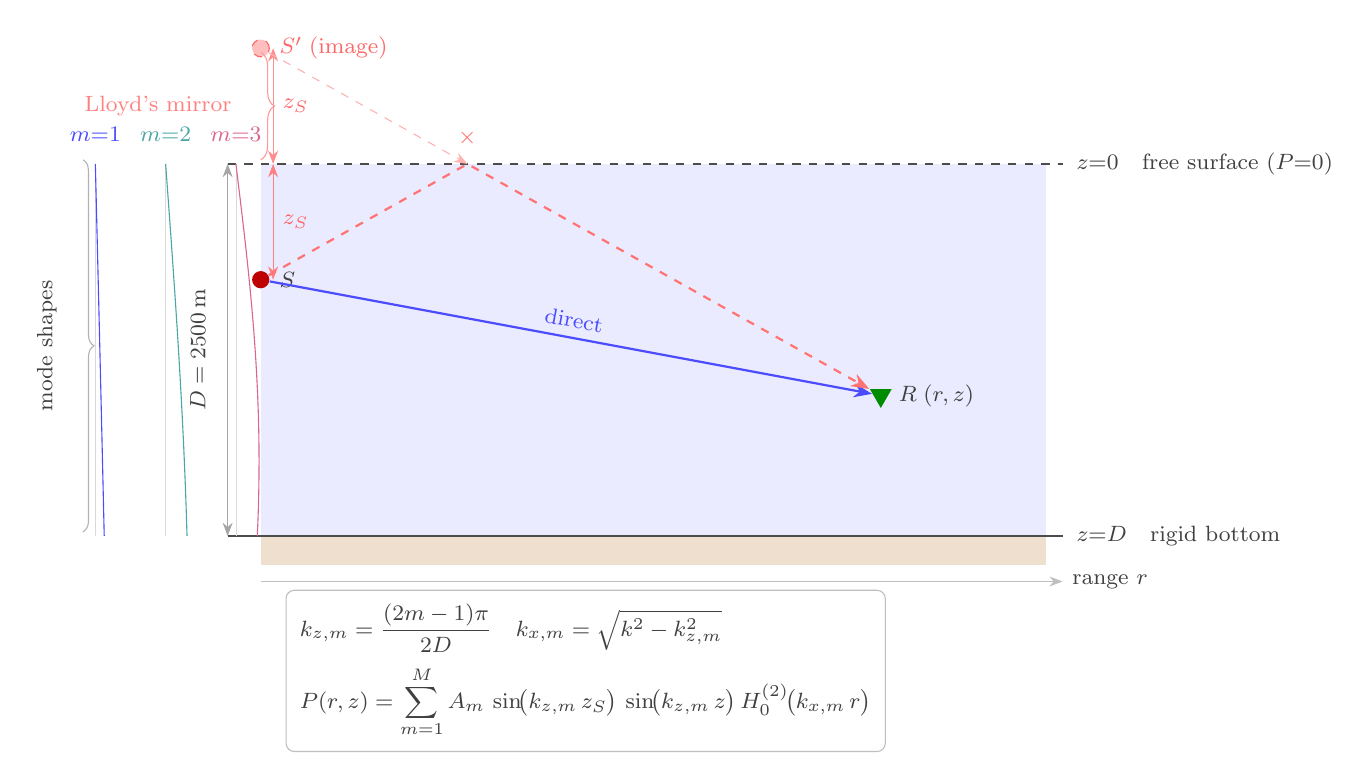
\begin{tikzpicture}[
    scale = 1.05,
    >=Stealth,
    every node/.style = {font=\small},
    % Named styles
    waterfill/.style = {fill=blue!8},
    sedfill/.style   = {fill=brown!25},
    surface/.style   = {dashed, thick, draw=black!70},
    bottom/.style    = {thick, draw=black!70},
    src/.style       = {circle, fill=red!75!black, inner sep=2.2pt},
    imgsrc/.style    = {circle, fill=red!25, draw=red!60, inner sep=2.2pt, dashed},
    rcv/.style       = {regular polygon, regular polygon sides=3, fill=green!55!black,
                        inner sep=1.6pt, rotate=180},
    ray/.style       = {->, thick},
    modeplot/.style  = {blue!60, thin, smooth},
    annot/.style     = {font=\footnotesize, text=black!75},
]

% ── Dimensions (tikz units; 1 unit ≈ 1 cm) ───────────────────────────────────
\def\D{4.5}     % waveguide depth  D
\def\Rmax{9.5}  % range extent
\def\zS{1.4}    % source depth  zS
\def\zR{2.8}    % receiver depth zR
\def\rR{7.5}    % receiver range rR

% ── Water column ──────────────────────────────────────────────────────────────
\fill[waterfill] (0,0) rectangle (\Rmax,-\D);
\fill[sedfill]   (0,-\D) rectangle (\Rmax,-\D-0.35);

% ── Boundaries ────────────────────────────────────────────────────────────────
% Free surface
\draw[surface] (-0.4,0) -- (\Rmax+0.2,0);
\node[right, annot] at (\Rmax+0.25, 0) {$z{=}0$\quad free surface ($P{=}0$)};

% Bottom
\draw[bottom]  (-0.4,-\D) -- (\Rmax+0.2,-\D);
\node[right, annot] at (\Rmax+0.25,-\D) {$z{=}D$\quad rigid bottom};

% Depth axis
\draw[<->, gray!70] (-0.4,0) -- (-0.4,-\D);
\node[left, annot, rotate=90, anchor=south] at (-0.55,-\D/2) {$D = 2500$\,m};

% Range axis
\draw[->, gray!50] (0,-\D-0.55) -- (\Rmax+0.2,-\D-0.55)
    node[right, annot] {range $r$};

% ── Image source (Lloyd's mirror) above surface ───────────────────────────────
\node[imgsrc, label={[annot,text=red!60]right:{$S'$\;(image)}}] (img) at (0,\zS) {};
% Bracket marking zS above surface
\draw[<->, red!45, thin] (0.15,0) -- (0.15,\zS)
    node[midway, right, annot, text=red!60] {$z_S$};

% ── Source ────────────────────────────────────────────────────────────────────
\node[src, label={[annot]right:{$S$}}] (src) at (0,-\zS) {};
\draw[<->, red!50, thin] (0.15,0) -- (0.15,-\zS)
    node[midway, right, annot, text=red!60] {$z_S$};

% ── Receiver ──────────────────────────────────────────────────────────────────
\node[rcv] (rcv) at (\rR,-\zR) {};
\node[annot, right=3pt] at (rcv) {$R\;(r,z)$};

% ── Rays ──────────────────────────────────────────────────────────────────────
% Direct ray
\draw[ray, blue!70]   (src) -- (rcv)
    node[midway, above, sloped, annot, text=blue!70] {direct};

% Surface-reflected ray (specular: image to receiver)
\pgfmathsetmacro{\xs}{\zS/(\zS+\zR)*\rR}
\coordinate (srf) at (\xs,0);
\draw[ray, red!55, dashed] (src) -- (srf) -- (rcv);
\node[annot, above=3pt, text=red!55] at (\xs,0) {$\times$};

% Arrow from image source to surface reflection point
\draw[->, red!30, thin, dashed] (img) -- (srf);

% Lloyd's mirror annotation
\draw[decorate, decoration={brace, amplitude=5pt, mirror}, red!40]
    (0, 0.05) -- (0, \zS-0.05)
    node[midway, left=7pt, annot, text=red!50] {Lloyd's mirror};

% ── Mode shape panel (right of waveguide) ─────────────────────────────────────
% Small panel showing sin((2m-1)*pi*z / (2D)) for m=1,2,3
% x_panel: right of the main figure
\def\Xpanel{-2.0}   % x offset into left margin
\def\ampmode{0.28}  % amplitude in tikz units

\foreach \m/\mcol in {1/blue!70, 2/teal!70, 3/purple!60} {
    % Baseline (zero line for this mode)
    \pgfmathsetmacro{\xbase}{\Xpanel + (\m-1)*0.85}
    \draw[gray!30, very thin] (\xbase, 0) -- (\xbase, -\D);
    % Sine curve: sin((2m-1)*22.5 * z) where z in [0,D] maps to y in [0,-D]
    \draw[\mcol, thin, smooth, samples=80,
          domain=0:\D]
        plot ({\xbase + \ampmode*sin((2*\m-1)*22.5/\D*\x)}, {-\x});
    % Mode label
    \node[annot, text=\mcol, above] at (\xbase, 0.15) {$m{=}\m$};
}
% Brace and label
\draw[decorate, decoration={brace, amplitude=4pt}, gray!60]
    (\Xpanel-0.15, 0.05) -- (\Xpanel-0.15, -\D+0.05)
    node[midway, left=6pt, annot, rotate=90, anchor=south] {mode shapes};

% ── Equation box ─────────────────────────────────────────────────────────────
\node[draw=gray!50, fill=white, rounded corners=3pt,
      inner sep=5pt, annot, align=left,
      anchor=north west] at (0.3, -\D-0.65) {%
  $k_{z,m} = \dfrac{(2m-1)\pi}{2D}$\quad
  $k_{x,m} = \sqrt{k^2 - k_{z,m}^2}$\\[4pt]
  $P(r,z) = \displaystyle\sum_{m=1}^{M}
             A_m\,
             \sin\!\bigl(k_{z,m}\,z_S\bigr)\,
             \sin\!\bigl(k_{z,m}\,z\bigr)\,
             H_0^{(2)}\!\bigl(k_{x,m}\,r\bigr)$
};

\end{tikzpicture}

%%   (wrap in a figure environment at the call site)

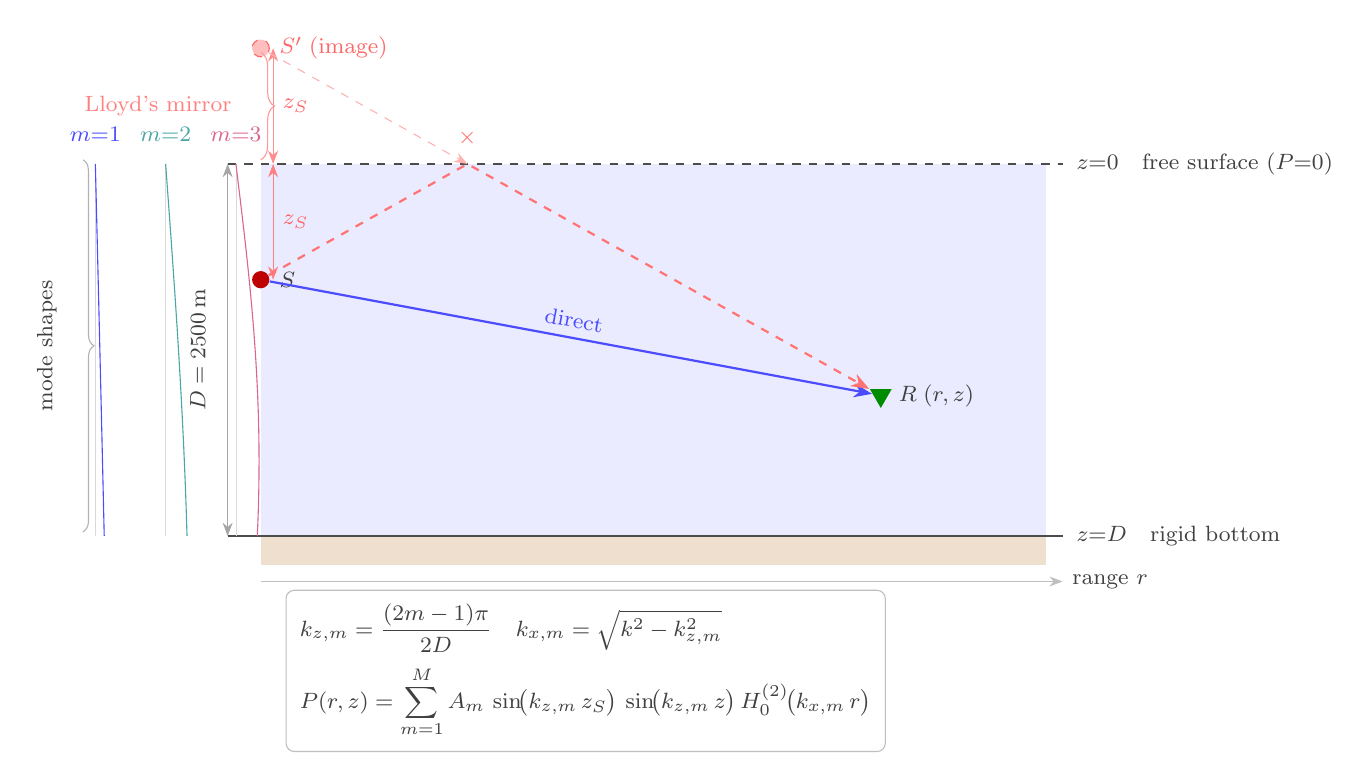
\begin{tikzpicture}[
    scale = 1.05,
    >=Stealth,
    every node/.style = {font=\small},
    % Named styles
    waterfill/.style = {fill=blue!8},
    sedfill/.style   = {fill=brown!25},
    surface/.style   = {dashed, thick, draw=black!70},
    bottom/.style    = {thick, draw=black!70},
    src/.style       = {circle, fill=red!75!black, inner sep=2.2pt},
    imgsrc/.style    = {circle, fill=red!25, draw=red!60, inner sep=2.2pt, dashed},
    rcv/.style       = {regular polygon, regular polygon sides=3, fill=green!55!black,
                        inner sep=1.6pt, rotate=180},
    ray/.style       = {->, thick},
    modeplot/.style  = {blue!60, thin, smooth},
    annot/.style     = {font=\footnotesize, text=black!75},
]

% ── Dimensions (tikz units; 1 unit ≈ 1 cm) ───────────────────────────────────
\def\D{4.5}     % waveguide depth  D
\def\Rmax{9.5}  % range extent
\def\zS{1.4}    % source depth  zS
\def\zR{2.8}    % receiver depth zR
\def\rR{7.5}    % receiver range rR

% ── Water column ──────────────────────────────────────────────────────────────
\fill[waterfill] (0,0) rectangle (\Rmax,-\D);
\fill[sedfill]   (0,-\D) rectangle (\Rmax,-\D-0.35);

% ── Boundaries ────────────────────────────────────────────────────────────────
% Free surface
\draw[surface] (-0.4,0) -- (\Rmax+0.2,0);
\node[right, annot] at (\Rmax+0.25, 0) {$z{=}0$\quad free surface ($P{=}0$)};

% Bottom
\draw[bottom]  (-0.4,-\D) -- (\Rmax+0.2,-\D);
\node[right, annot] at (\Rmax+0.25,-\D) {$z{=}D$\quad rigid bottom};

% Depth axis
\draw[<->, gray!70] (-0.4,0) -- (-0.4,-\D);
\node[left, annot, rotate=90, anchor=south] at (-0.55,-\D/2) {$D = 2500$\,m};

% Range axis
\draw[->, gray!50] (0,-\D-0.55) -- (\Rmax+0.2,-\D-0.55)
    node[right, annot] {range $r$};

% ── Image source (Lloyd's mirror) above surface ───────────────────────────────
\node[imgsrc, label={[annot,text=red!60]right:{$S'$\;(image)}}] (img) at (0,\zS) {};
% Bracket marking zS above surface
\draw[<->, red!45, thin] (0.15,0) -- (0.15,\zS)
    node[midway, right, annot, text=red!60] {$z_S$};

% ── Source ────────────────────────────────────────────────────────────────────
\node[src, label={[annot]right:{$S$}}] (src) at (0,-\zS) {};
\draw[<->, red!50, thin] (0.15,0) -- (0.15,-\zS)
    node[midway, right, annot, text=red!60] {$z_S$};

% ── Receiver ──────────────────────────────────────────────────────────────────
\node[rcv] (rcv) at (\rR,-\zR) {};
\node[annot, right=3pt] at (rcv) {$R\;(r,z)$};

% ── Rays ──────────────────────────────────────────────────────────────────────
% Direct ray
\draw[ray, blue!70]   (src) -- (rcv)
    node[midway, above, sloped, annot, text=blue!70] {direct};

% Surface-reflected ray (specular: image to receiver)
\pgfmathsetmacro{\xs}{\zS/(\zS+\zR)*\rR}
\coordinate (srf) at (\xs,0);
\draw[ray, red!55, dashed] (src) -- (srf) -- (rcv);
\node[annot, above=3pt, text=red!55] at (\xs,0) {$\times$};

% Arrow from image source to surface reflection point
\draw[->, red!30, thin, dashed] (img) -- (srf);

% Lloyd's mirror annotation
\draw[decorate, decoration={brace, amplitude=5pt, mirror}, red!40]
    (0, 0.05) -- (0, \zS-0.05)
    node[midway, left=7pt, annot, text=red!50] {Lloyd's mirror};

% ── Mode shape panel (right of waveguide) ─────────────────────────────────────
% Small panel showing sin((2m-1)*pi*z / (2D)) for m=1,2,3
% x_panel: right of the main figure
\def\Xpanel{-2.0}   % x offset into left margin
\def\ampmode{0.28}  % amplitude in tikz units

\foreach \m/\mcol in {1/blue!70, 2/teal!70, 3/purple!60} {
    % Baseline (zero line for this mode)
    \pgfmathsetmacro{\xbase}{\Xpanel + (\m-1)*0.85}
    \draw[gray!30, very thin] (\xbase, 0) -- (\xbase, -\D);
    % Sine curve: sin((2m-1)*22.5 * z) where z in [0,D] maps to y in [0,-D]
    \draw[\mcol, thin, smooth, samples=80,
          domain=0:\D]
        plot ({\xbase + \ampmode*sin((2*\m-1)*22.5/\D*\x)}, {-\x});
    % Mode label
    \node[annot, text=\mcol, above] at (\xbase, 0.15) {$m{=}\m$};
}
% Brace and label
\draw[decorate, decoration={brace, amplitude=4pt}, gray!60]
    (\Xpanel-0.15, 0.05) -- (\Xpanel-0.15, -\D+0.05)
    node[midway, left=6pt, annot, rotate=90, anchor=south] {mode shapes};

% ── Equation box ─────────────────────────────────────────────────────────────
\node[draw=gray!50, fill=white, rounded corners=3pt,
      inner sep=5pt, annot, align=left,
      anchor=north west] at (0.3, -\D-0.65) {%
  $k_{z,m} = \dfrac{(2m-1)\pi}{2D}$\quad
  $k_{x,m} = \sqrt{k^2 - k_{z,m}^2}$\\[4pt]
  $P(r,z) = \displaystyle\sum_{m=1}^{M}
             A_m\,
             \sin\!\bigl(k_{z,m}\,z_S\bigr)\,
             \sin\!\bigl(k_{z,m}\,z\bigr)\,
             H_0^{(2)}\!\bigl(k_{x,m}\,r\bigr)$
};

\end{tikzpicture}

%%   (wrap in a figure environment at the call site)

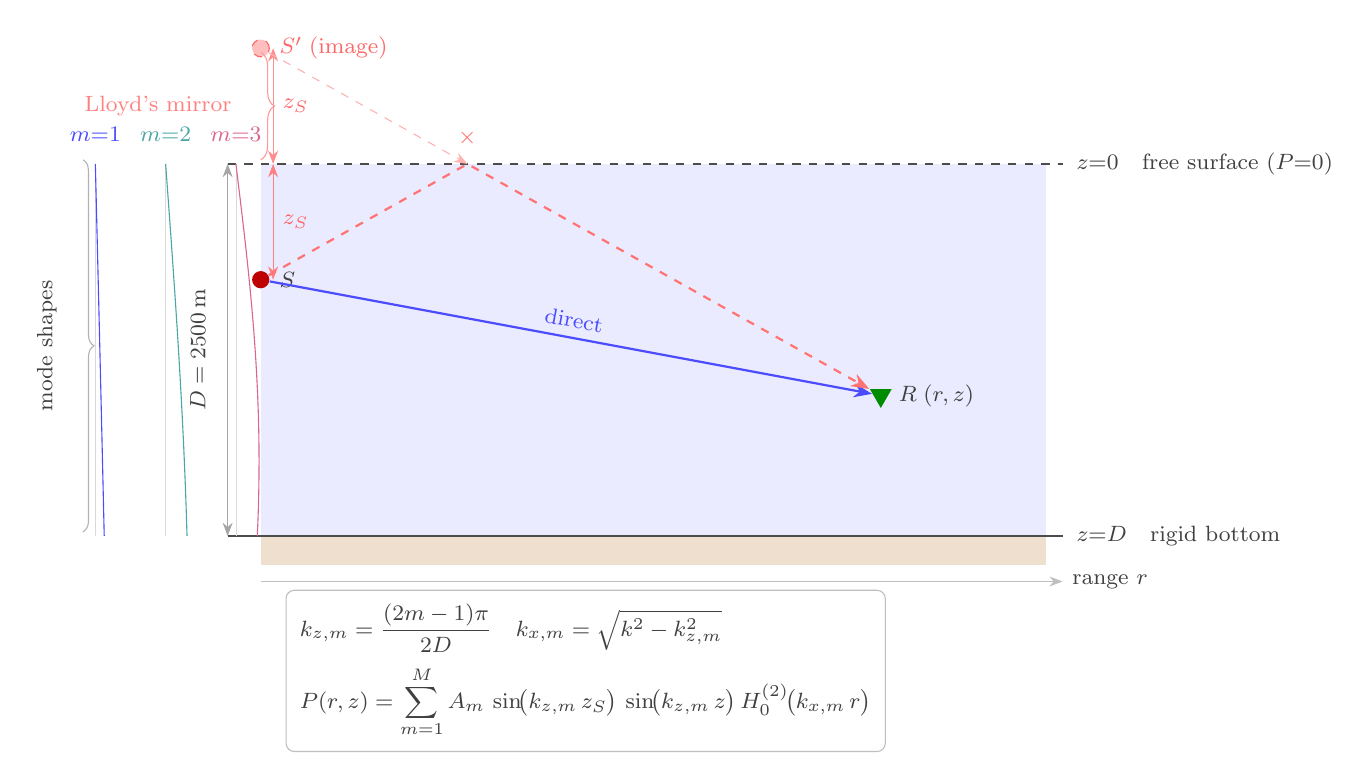
\begin{tikzpicture}[
    scale = 1.05,
    >=Stealth,
    every node/.style = {font=\small},
    % Named styles
    waterfill/.style = {fill=blue!8},
    sedfill/.style   = {fill=brown!25},
    surface/.style   = {dashed, thick, draw=black!70},
    bottom/.style    = {thick, draw=black!70},
    src/.style       = {circle, fill=red!75!black, inner sep=2.2pt},
    imgsrc/.style    = {circle, fill=red!25, draw=red!60, inner sep=2.2pt, dashed},
    rcv/.style       = {regular polygon, regular polygon sides=3, fill=green!55!black,
                        inner sep=1.6pt, rotate=180},
    ray/.style       = {->, thick},
    modeplot/.style  = {blue!60, thin, smooth},
    annot/.style     = {font=\footnotesize, text=black!75},
]

% ── Dimensions (tikz units; 1 unit ≈ 1 cm) ───────────────────────────────────
\def\D{4.5}     % waveguide depth  D
\def\Rmax{9.5}  % range extent
\def\zS{1.4}    % source depth  zS
\def\zR{2.8}    % receiver depth zR
\def\rR{7.5}    % receiver range rR

% ── Water column ──────────────────────────────────────────────────────────────
\fill[waterfill] (0,0) rectangle (\Rmax,-\D);
\fill[sedfill]   (0,-\D) rectangle (\Rmax,-\D-0.35);

% ── Boundaries ────────────────────────────────────────────────────────────────
% Free surface
\draw[surface] (-0.4,0) -- (\Rmax+0.2,0);
\node[right, annot] at (\Rmax+0.25, 0) {$z{=}0$\quad free surface ($P{=}0$)};

% Bottom
\draw[bottom]  (-0.4,-\D) -- (\Rmax+0.2,-\D);
\node[right, annot] at (\Rmax+0.25,-\D) {$z{=}D$\quad rigid bottom};

% Depth axis
\draw[<->, gray!70] (-0.4,0) -- (-0.4,-\D);
\node[left, annot, rotate=90, anchor=south] at (-0.55,-\D/2) {$D = 2500$\,m};

% Range axis
\draw[->, gray!50] (0,-\D-0.55) -- (\Rmax+0.2,-\D-0.55)
    node[right, annot] {range $r$};

% ── Image source (Lloyd's mirror) above surface ───────────────────────────────
\node[imgsrc, label={[annot,text=red!60]right:{$S'$\;(image)}}] (img) at (0,\zS) {};
% Bracket marking zS above surface
\draw[<->, red!45, thin] (0.15,0) -- (0.15,\zS)
    node[midway, right, annot, text=red!60] {$z_S$};

% ── Source ────────────────────────────────────────────────────────────────────
\node[src, label={[annot]right:{$S$}}] (src) at (0,-\zS) {};
\draw[<->, red!50, thin] (0.15,0) -- (0.15,-\zS)
    node[midway, right, annot, text=red!60] {$z_S$};

% ── Receiver ──────────────────────────────────────────────────────────────────
\node[rcv] (rcv) at (\rR,-\zR) {};
\node[annot, right=3pt] at (rcv) {$R\;(r,z)$};

% ── Rays ──────────────────────────────────────────────────────────────────────
% Direct ray
\draw[ray, blue!70]   (src) -- (rcv)
    node[midway, above, sloped, annot, text=blue!70] {direct};

% Surface-reflected ray (specular: image to receiver)
\pgfmathsetmacro{\xs}{\zS/(\zS+\zR)*\rR}
\coordinate (srf) at (\xs,0);
\draw[ray, red!55, dashed] (src) -- (srf) -- (rcv);
\node[annot, above=3pt, text=red!55] at (\xs,0) {$\times$};

% Arrow from image source to surface reflection point
\draw[->, red!30, thin, dashed] (img) -- (srf);

% Lloyd's mirror annotation
\draw[decorate, decoration={brace, amplitude=5pt, mirror}, red!40]
    (0, 0.05) -- (0, \zS-0.05)
    node[midway, left=7pt, annot, text=red!50] {Lloyd's mirror};

% ── Mode shape panel (right of waveguide) ─────────────────────────────────────
% Small panel showing sin((2m-1)*pi*z / (2D)) for m=1,2,3
% x_panel: right of the main figure
\def\Xpanel{-2.0}   % x offset into left margin
\def\ampmode{0.28}  % amplitude in tikz units

\foreach \m/\mcol in {1/blue!70, 2/teal!70, 3/purple!60} {
    % Baseline (zero line for this mode)
    \pgfmathsetmacro{\xbase}{\Xpanel + (\m-1)*0.85}
    \draw[gray!30, very thin] (\xbase, 0) -- (\xbase, -\D);
    % Sine curve: sin((2m-1)*22.5 * z) where z in [0,D] maps to y in [0,-D]
    \draw[\mcol, thin, smooth, samples=80,
          domain=0:\D]
        plot ({\xbase + \ampmode*sin((2*\m-1)*22.5/\D*\x)}, {-\x});
    % Mode label
    \node[annot, text=\mcol, above] at (\xbase, 0.15) {$m{=}\m$};
}
% Brace and label
\draw[decorate, decoration={brace, amplitude=4pt}, gray!60]
    (\Xpanel-0.15, 0.05) -- (\Xpanel-0.15, -\D+0.05)
    node[midway, left=6pt, annot, rotate=90, anchor=south] {mode shapes};

% ── Equation box ─────────────────────────────────────────────────────────────
\node[draw=gray!50, fill=white, rounded corners=3pt,
      inner sep=5pt, annot, align=left,
      anchor=north west] at (0.3, -\D-0.65) {%
  $k_{z,m} = \dfrac{(2m-1)\pi}{2D}$\quad
  $k_{x,m} = \sqrt{k^2 - k_{z,m}^2}$\\[4pt]
  $P(r,z) = \displaystyle\sum_{m=1}^{M}
             A_m\,
             \sin\!\bigl(k_{z,m}\,z_S\bigr)\,
             \sin\!\bigl(k_{z,m}\,z\bigr)\,
             H_0^{(2)}\!\bigl(k_{x,m}\,r\bigr)$
};

\end{tikzpicture}

  \caption{Isovelocity waveguide geometry used for analytical validation.
           Source $S$ at depth $z_S$ and its pressure-release image $S'$
           at $-z_S$ form a dipole (Lloyd's mirror) whose radiation pattern
           imposes a depth-dependent modulation on the cylindrical spreading.
           Mode shapes $\sin(k_{z,m}\,z)$ (shown for $m=1,2,3$, colour-coded)
           satisfy the pressure-release condition at $z=0$ and rigid-bottom
           condition at $z=D$.
           The horizontal wavenumbers $k_{x,m}$ set the along-range interference
           structure that makes the analytical Jacobian $\partial\TL/\partial z_S$
           highly oscillatory at long range.}
  \label{fig:waveguide_diagram}
\end{figure}

The analytical Jacobian is:
\begin{equation}
  J^{\mathrm{anal}} = -\frac{20}{\ln 10}
  \;\frac{\mathrm{Re}\!\left[P^*\,\partial P/\partial z_S\right]}{|P|^2},
  \qquad
  \frac{\partial P}{\partial z_S} = \sum_m N_m\,k_{z,m}\cos(k_{z,m} z_S)\,\psi_m(z,r)
\end{equation}
where $N_m$, $k_{z,m}$, and $\psi_m$ are the mode normalisation, vertical
wavenumber, and field shape of the $m$-th normal mode.
The finite-difference (FD) Jacobian used in the numerical pipeline matches the
analytical Jacobian to 8.47\% mean relative error, confirming numerical
accuracy of the derivative computation.

\begin{figure}[H]
  \centering
  \begin{subfigure}[t]{0.48\textwidth}
    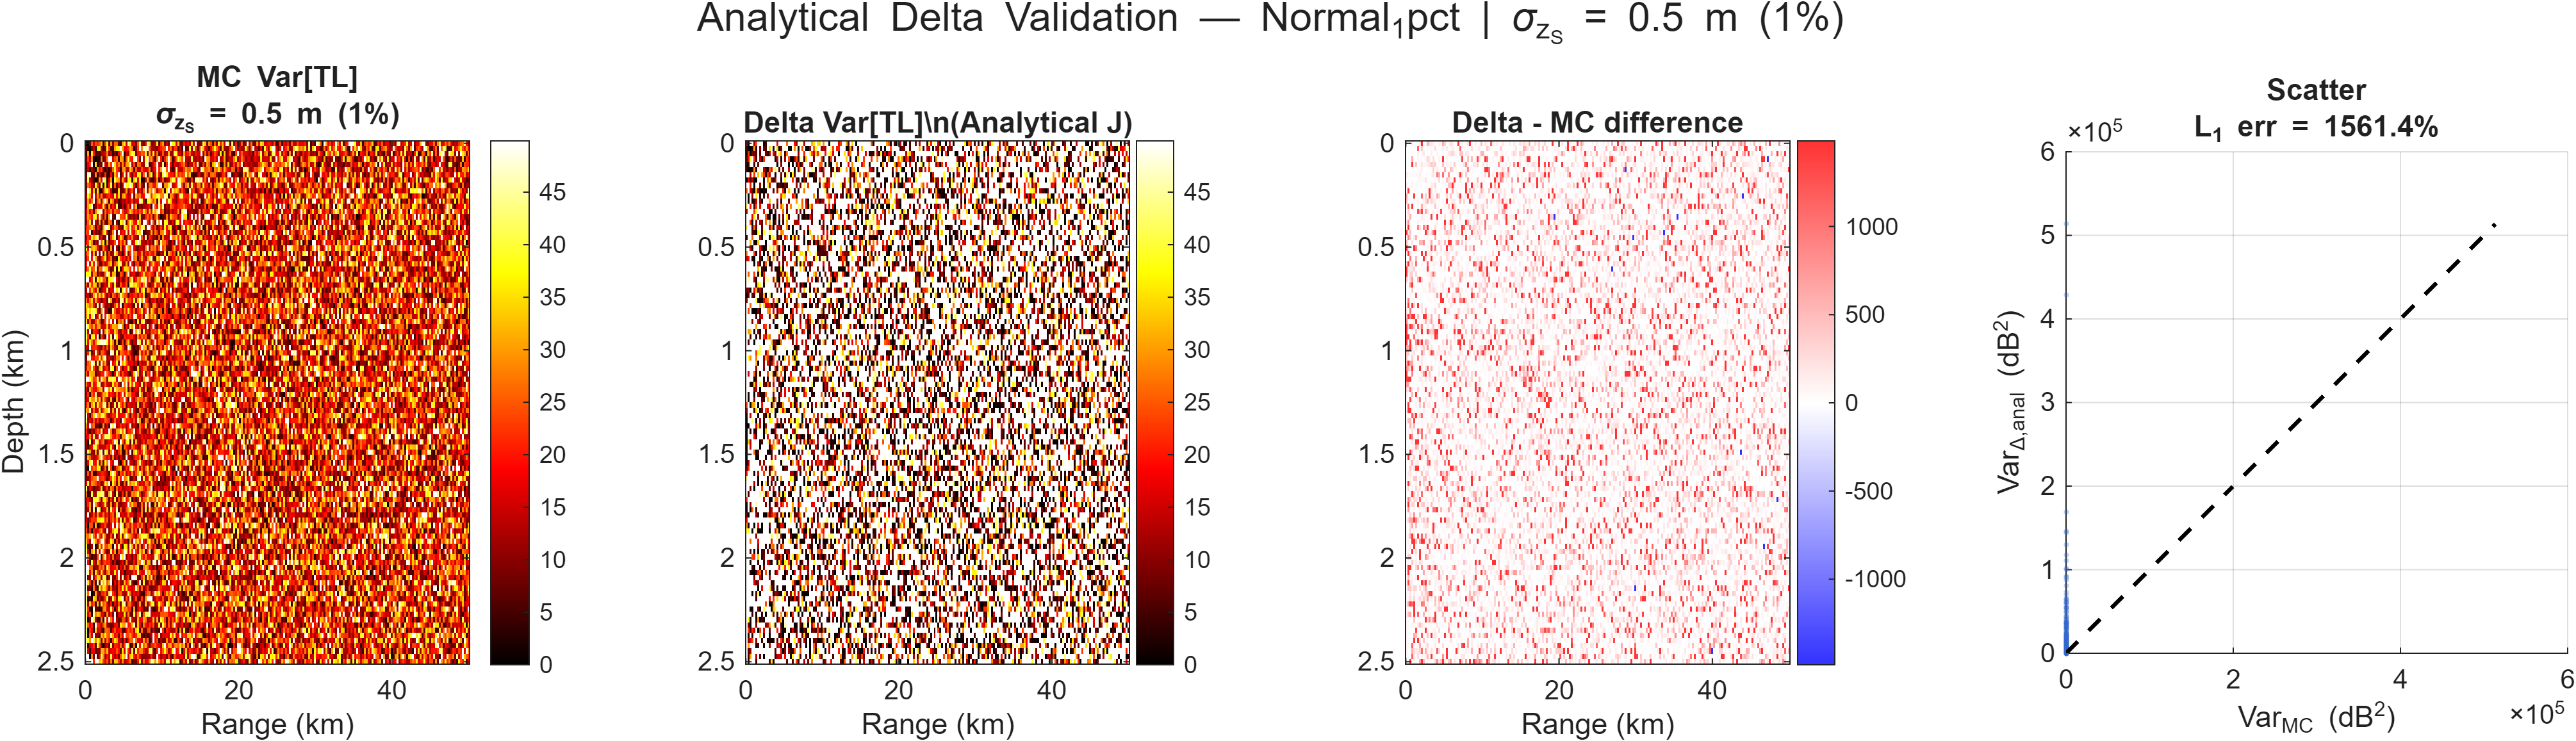
\includegraphics[width=\linewidth]{delta_validation_Normal_1pct.png}
    \caption{Normal\,1\% ($\sigma_{z_S}=0.5$\,m)}
  \end{subfigure}\hfill
  \begin{subfigure}[t]{0.48\textwidth}
    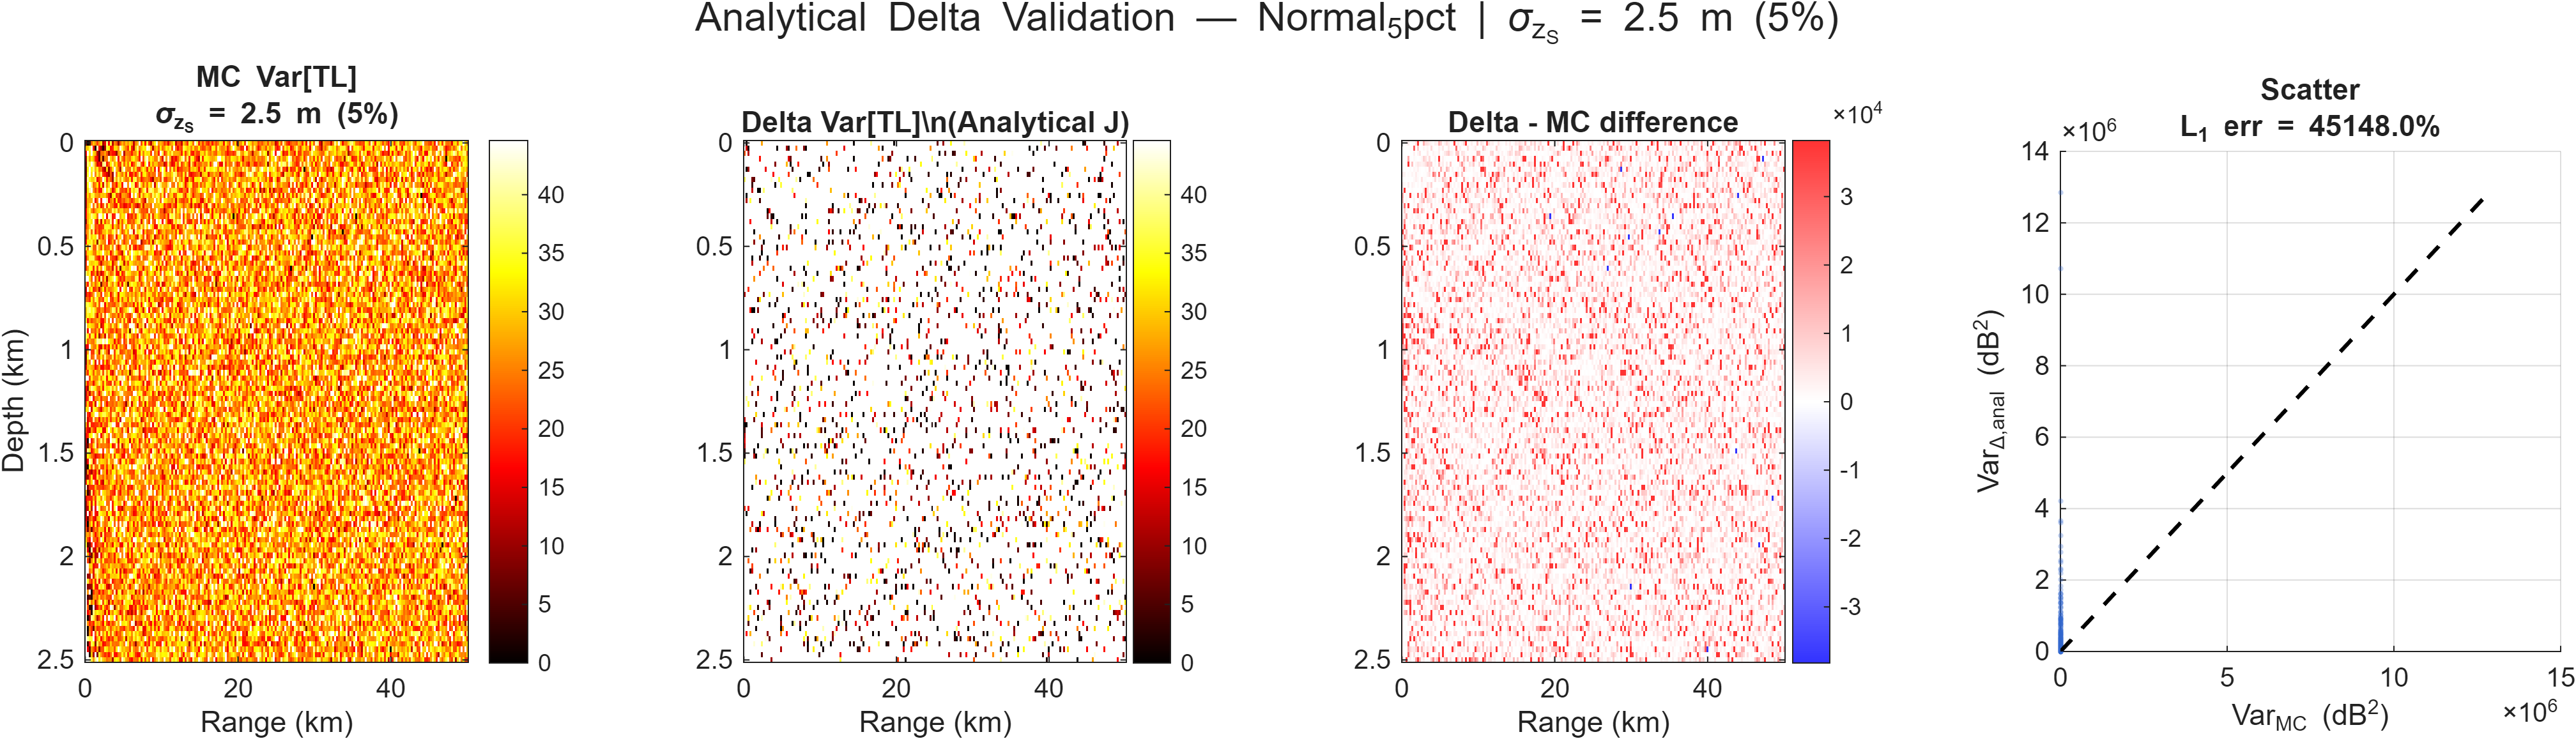
\includegraphics[width=\linewidth]{delta_validation_Normal_5pct.png}
    \caption{Normal\,5\% ($\sigma_{z_S}=2.5$\,m)}
  \end{subfigure}\\[8pt]
  \begin{subfigure}[t]{0.48\textwidth}
    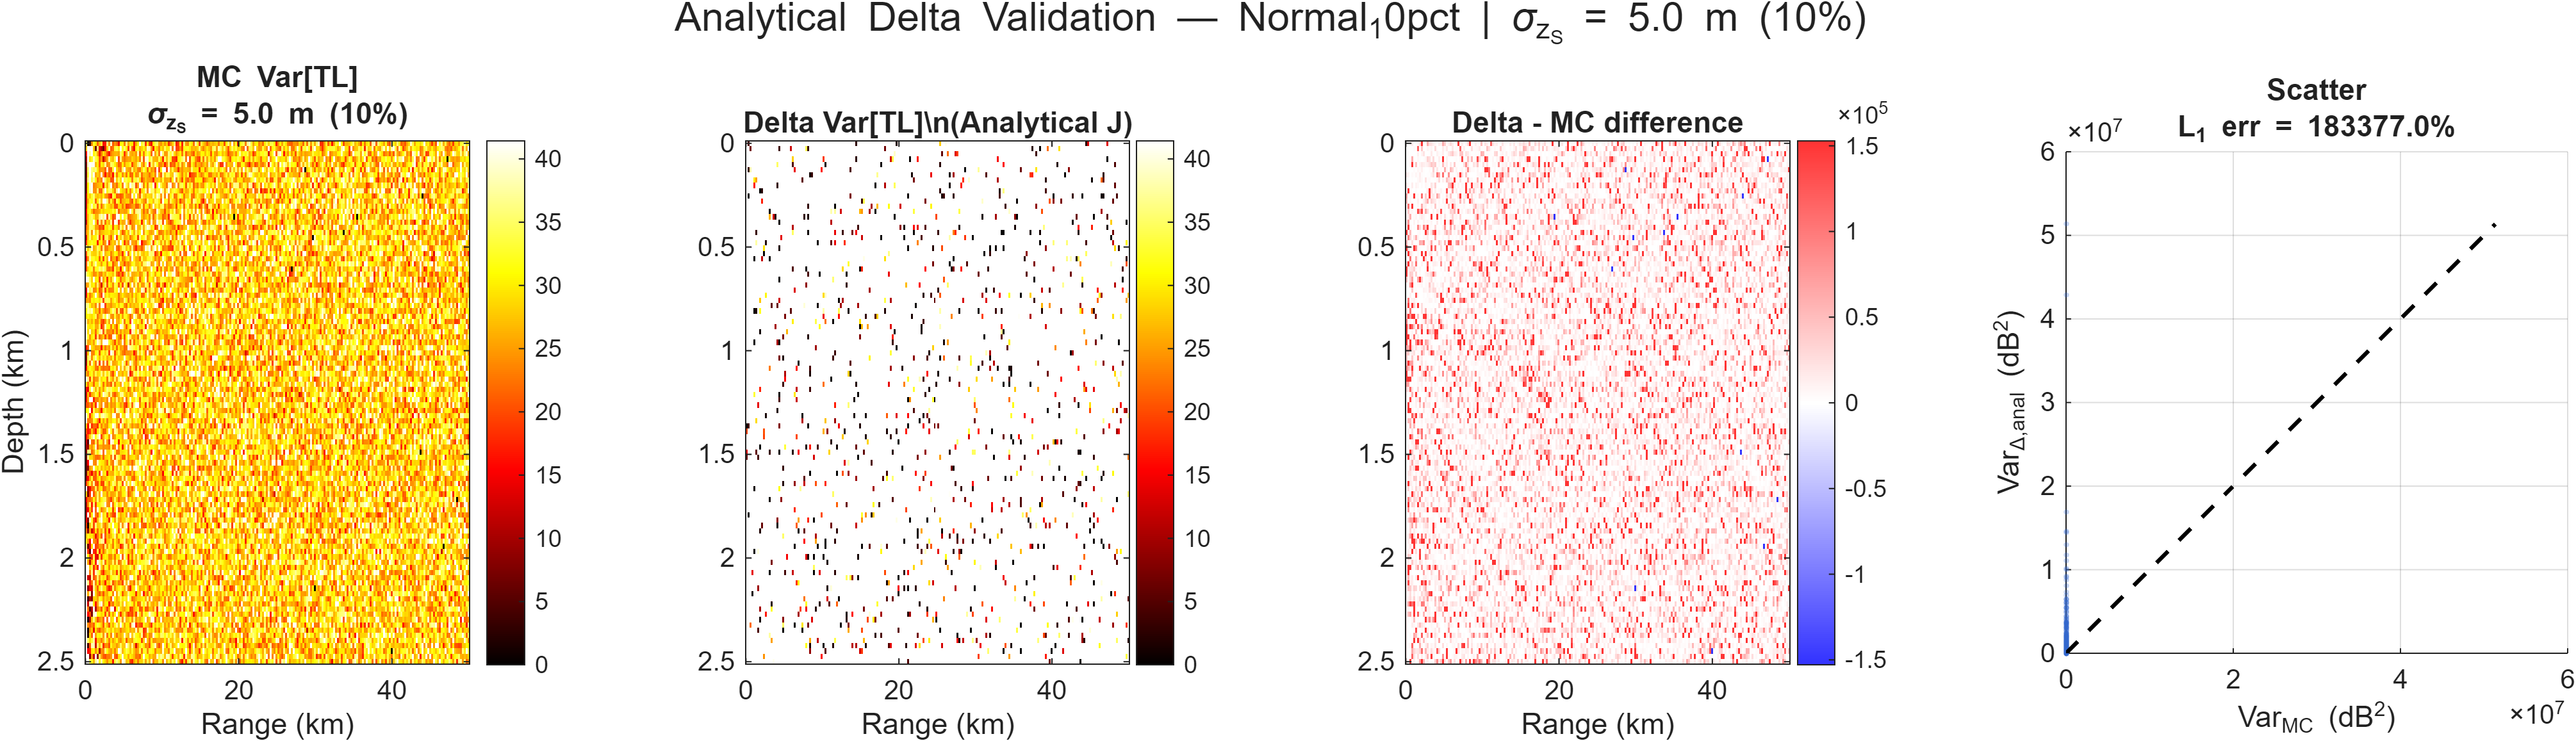
\includegraphics[width=\linewidth]{delta_validation_Normal_10pct.png}
    \caption{Normal\,10\% ($\sigma_{z_S}=5$\,m)}
  \end{subfigure}
  \caption{Analytical Delta validation. Columns: $\Var_\text{MC}$ / $\Var_{\Delta,\text{anal}}$ /
           difference map / scatter. Masked to TL\,$\leq$\,120\,dB (excluding interference nulls).}
  \label{fig:analytical}
\end{figure}

\begin{table}[H]
  \centering
  \caption{Relative $L_1$ error of 1\textsuperscript{st}-order Delta variance vs
           analytical MC ground truth (deep-water waveguide, $f=1$\,kHz, $z_S=100$\,m,
           $N_{\rm MC}=2000$).
           $L_1 = \langle|\mathrm{Var}_\Delta - \mathrm{Var}_{\rm MC}|\rangle /
           \langle\mathrm{Var}_{\rm MC}\rangle$ (dimensionless ratio; values $\gg 1$ indicate
           Delta breakdown).}
  \label{tab:analytical_l1}
  \begin{tabular}{lccc}
    \toprule
    Distribution & $\sigma_{z_S}$ (m) & $L_1$ (Analytical $J$) & $L_1$ (FD $J$) \\
    \midrule
    Normal\,1\%  & 0.5 & 24.2  & 16.2  \\
    Normal\,5\%  & 2.5 & 494   & 336   \\
    Normal\,10\% & 5.0 & 1922  & 1306  \\
    \bottomrule
  \end{tabular}
\end{table}

% ────────────────────────────────────────────────────────────
\subsection{Summary of Findings}
\label{sec:summary}

\begin{table}[H]
  \centering
  \caption{Recommended UQ method by scenario and uncertainty level.}
  \label{tab:recommendation}
  \begin{tabular}{llll}
    \toprule
    Scenario & Small ($\leq$1\%) & Medium (5\%) & Large (10\%) \\
    \midrule
    Baseline (flat, 50\,m)   & Delta 1\textsuperscript{st}  & Delta 2\textsuperscript{nd} / PCE-2 & PCE-$K^*$ \\
    Deep water (flat, 2500\,m)   & Delta 1\textsuperscript{st}  & PCE-3                               & PCE-$K^*$ or MC \\
    Shallow water (flat, 50\,m)  & Delta 1\textsuperscript{st}  & PCE-3--5                            & MC \\
    Upslope / Downslope          & Delta 2\textsuperscript{nd}  & PCE-5+                              & MC \\
    \bottomrule
  \end{tabular}
\end{table}

Taken together, the results show a clear hierarchy of method applicability
determined by two physical factors: \emph{bathymetric complexity} (flat vs
slope) and \emph{perturbation magnitude} ($\leq$1\% vs 5--10\%).
For flat environments with small perturbations the acoustic field is nearly
linear in all three uncertain parameters, so the cheap Delta approximation
suffices.  As perturbations grow, the nonlinearity of the interference pattern
(especially in deep water) requires a higher-order representation; PCE fills
this gap without any new Bellhop runs.  Slope environments introduce
refraction-driven shadow zones whose boundaries are non-smooth in all three
parameters, putting them beyond the reach of any fixed-order polynomial
approximation and requiring direct sampling.  From a sonar-planning perspective,
the most operationally useful outputs are not variance maps but
$P_\mathrm{fail}$ maps (probability that TL exceeds the sonar Figure-of-Merit)
and P95 TL envelopes, both of which reveal the \emph{direction} of uncertainty
in a way that variance alone does not.

Key findings are:
\begin{enumerate}
  \item The 1\textsuperscript{st}-order Delta method is accurate for flat bathymetry
        at low uncertainty ($\leq$1\%) but the 2\textsuperscript{nd}-order Hessian
        correction already exceeds 96\% of the total variance for 5\% uncertainty
        across all scenarios, indicating that the Taylor series has not converged
        at order~2.
  \item Shadow-probability maps from the Delta--LN3 hybrid are reliable for flat-bottom
        scenarios but fail at shadow-zone boundaries in slope environments, where
        the acoustic field is highly sensitive to bathymetric refraction.
  \item PCE with Gauss quadrature provides a systematic path from the 1\textsuperscript{st}-order
        Delta approximation to the full MC reference: each additional order requires
        only one extra Bellhop evaluation per parameter, with guaranteed monotone
        convergence for smooth TL responses.
  \item For strongly nonlinear scenarios (slope bathymetry, $\geq$5\% SVP uncertainty),
        no polynomial expansion of order $\leq$10 achieves $L_1 < 10\%$, confirming
        that full Monte Carlo simulation is necessary in these regimes.
  \item The analytical waveguide study confirms that the FD Jacobian used in the
        numerical pipeline has 8.47\% mean error relative to the exact derivative,
        validating the Bellhop-based Delta method implementation.
  \item The LN3 distribution fitting strategy (method of moments) is a known
        methodological weakness.  Maximum likelihood estimation (MLE) would be
        statistically superior, but the LHS samples used throughout this pipeline
        are not i.i.d.: LHS stratification introduces negative inter-stratum
        correlations that violate the independence assumption of the standard MLE
        log-likelihood.  Applying i.i.d.\ MLE to LHS samples would yield biased
        parameter uncertainty estimates.  Correcting this requires a
        design-weighted or survey-sampling pseudo-likelihood, which is left for
        future work.
\end{enumerate}

% ============================================================
\section{Related Work and Literature Comparison}
\label{sec:related}

% ────────────────────────────────────────────────────────────
\subsection{Summary of Related Papers}
\label{sec:papers}

Four papers from the stochastic underwater acoustics literature are directly
relevant to this work.

\paragraph{Finette~(2009) — PCE for Acoustic Propagation Uncertainty.}
The paper \emph{Estimation of Acoustic Propagation Uncertainty Through Polynomial
Chaos Expansions} establishes the canonical framework for applying PCE to
underwater TL estimation.
Using probabilist Hermite polynomials for Gaussian sound-speed perturbations
and a Gauss–Hermite quadrature grid rather than a Monte Carlo regression fit,
Finette reports that $K = 3$--$5$ suffices to capture variance in a deep-water
isovelocity waveguide under SVP uncertainty.
Convergence degrades for larger perturbations ($>$5\%) and near shadow-zone
boundaries where the pressure field is non-smooth.
The paper focuses on variance as the primary metric, with brief discussion of
probability density shapes (approximately Gaussian far from shadow zones).

\paragraph{East China Sea Sonar Performance Paper.}
The paper \emph{Acoustic Propagation Uncertainty and Probabilistic Prediction of
Sonar System Performance in the Southern East China Sea Continental Shelf and
Shelfbreak Environments} applies ensemble Monte Carlo methods to realistic
environmental uncertainty in a shelf/shelfbreak setting.
Uncertain parameters are the full sound-speed profile (temperature/salinity
variability) and bathymetric uncertainty; source/receiver geometry is treated
as fixed.
Key finding: the shelfbreak transition zone produces dramatically higher acoustic
uncertainty than the flat shelf, driven by modal cut-off sensitivity.
The paper computes detection probability as a function of Figure-of-Merit threshold,
going beyond variance to an operationally meaningful metric.

\paragraph{Reduced-Order Machine-Learning Surrogate.}
The paper \emph{Reduced-Order Machine-Learning Model for Transmission Loss
Prediction in Underwater Acoustics} replaces the Bellhop propagation model with
a neural-network or Gaussian-process surrogate trained on a large corpus of
simulations (hundreds to thousands of samples).
Once trained, the surrogate enables near-instantaneous TL prediction and variance
estimation under environmental uncertainty.
The approach reports surrogate prediction errors of 1--3\,dB RMSE, comparable to
Bellhop's own numerical accuracy.
Unlike our PCE regression (which uses \emph{the same} $N=50$ MC samples as the
MC reference), the surrogate approach requires a separate training dataset.

\paragraph{JMSE-10-01548.}
This \emph{Journal of Marine Science and Engineering} paper (2022) addresses
probabilistic sonar performance in a realistic ocean environment, combining
Delta/sensitivity analysis with MC validation and exceedance-probability maps.
It explicitly treats frequency, source depth, and SVP as uncertain parameters —
mirroring our three-parameter setup — and discusses the limitations of first-order
Delta methods at range-dependent bathymetry.

% ────────────────────────────────────────────────────────────
\subsection{Direct Comparison: Their Results vs.\ Ours}
\label{sec:comparison}

\begin{table}[H]
  \centering
  \caption{Side-by-side comparison of PCE convergence orders and key methodological choices.}
  \label{tab:lit_comparison}
  \begin{tabular}{lccl}
    \toprule
    Aspect & Literature & This work & Notes \\
    \midrule
    PCE basis & Hermite / Legendre & Hermite / Legendre & Same \\
    Coefficient method & Gauss quadrature & QR least-squares regression & Different \\
    Samples for PCE & Gauss nodes (few) & $N=50$ LHS (repurposed MC) & Ours: zero new runs \\
    SVP conv.\ order (deep) & $K^* = 3$--$5$ & $K^* = 4$--$6$ & Comparable \\
    $z_S$ conv.\ (deep, large $\sigma$) & Not reported & $K^* > 10$ & Our gap \\
    Freq conv.\ order & Not primary focus & $K^* = 1$--$9$ & New in this work \\
    Slope environments & Not covered & $K^* > 10$ (svp, freq) & New in this work \\
    Sobol indices & Not computed & Approx.\ via 1-D PCE & Partial \\
    Beyond-variance metrics & PDF shapes only & P95, P(fail), CI90 & Extended here \\
    Cross-validation & Not discussed & Task B below & New in this work \\
    \bottomrule
  \end{tabular}
\end{table}

\paragraph{Where results agree.}
Our SVP convergence orders for deep-water flat bathymetry ($K^* = 4$--$6$ for 5--10\%
Normal uncertainty) are consistent with the 3--5 orders reported by Finette (2009),
confirming that our regression-based PCE implementation is correctly calibrated.
The finding that slope environments resist polynomial convergence is consistent with
the East China Sea paper's observation that shelfbreak acoustic uncertainty is much
harder to model than flat-shelf uncertainty.

\paragraph{Where results differ or extend.}
\begin{itemize}
  \item \textbf{Source depth ($z_S$) convergence.} The PCE literature focuses almost
        exclusively on SVP as the dominant uncertain parameter.  Our study finds that
        $z_S$ is equally or more problematic: $K^* > 10$ for all Normal distributions
        in deep water, and for all distributions in the shallow-water scenario.
        This has not been quantified in the referenced papers.
  \item \textbf{Frequency uncertainty.} Treating frequency as a stochastic variable
        is not standard in the PCE acoustic literature.  Our results show $K^* = 1$--$9$
        depending on scenario and perturbation level, with the shallow-water scenario being the
        most benign (always $K^* = 1$).  This is a new contribution.
  \item \textbf{Regression vs.\ quadrature.} The Finette (2009) approach requires
        choosing Gauss quadrature nodes \emph{before} running simulations.  Our
        approach reuses existing LHS MC samples, which is more flexible but
        statistically less efficient.  The cross-validation analysis in
        Section~\ref{sec:cv} quantifies the cost of this flexibility.
  \item \textbf{1st-order Delta accuracy.}  The JMSE-10-01548 paper confirms our
        finding that the first-order Delta method fails at slope environments, and
        the 2nd-order Hessian correction does not recover the deficit — consistent
        with our Table~\ref{tab:2nd_order_correction} showing $>$96\% correction
        fraction in most scenarios.
\end{itemize}

\paragraph{What we missed compared to the literature.}
\begin{itemize}
  \item \textbf{Multi-parameter joint PCE.} The papers (and PCE theory) support
        full tensor-product or sparse-grid multi-parameter PCE, which captures
        interaction terms ($S_{z_S,\mathrm{svp}}$, etc.).  Our 1-D per-parameter
        approach assumes parameters enter independently, which is an approximation
        (see Section~\ref{sec:sobol}).
  \item \textbf{Gauss quadrature coefficient fitting.} With dedicated quadrature
        nodes, PCE coefficients are computed exactly without solving a regression
        problem, avoiding the overfitting risk discussed in Section~\ref{sec:cv}.
  \item \textbf{Sparse PCE / LARS.}  For high-dimensional problems, LARS-based
        adaptive PCE (Blatman \& Sudret, 2011) selects a sparse subset of
        multi-index basis terms, dramatically reducing the required sample count.
  \item \textbf{Operational sonar metrics.}  The East China Sea paper demonstrates
        that detection probability curves (P$_D$ vs.\ range) are the most useful
        output for sonar operators.  We compute P(TL\,$>$\,threshold) in
        Section~\ref{sec:metrics} but do not integrate it with the sonar FOM framework.
\end{itemize}

\paragraph{Future work suggested by the literature.}
\begin{enumerate}
  \item Implement multi-parameter sparse PCE using LARS with cross-validation for
        order/sparsity selection.
  \item Use Gauss quadrature nodes (pre-planned) rather than LHS for PCE coefficient
        fitting, reducing the required sample count.
  \item Compute full first- and total-order Sobol indices from the joint PCE to
        identify dominant and interaction uncertainty sources.
  \item Extend to realistic ocean environments (range-dependent SVP, measured
        bathymetry) and validate against operational sonar performance data.
\end{enumerate}

% ────────────────────────────────────────────────────────────
\subsection{PCE Overfitting and Cross-Validation}
\label{sec:cv}

\subsubsection{Theoretical Concern}

With $N=50$ MC samples and PCE order up to $K=10$, the regression design matrix
$\boldsymbol\Phi \in \mathbb{R}^{50 \times (K+1)}$ has $K+1 = 11$ columns at maximum
order.  The effective degrees of freedom ratio is $N/(K+1) \approx 4.5$, which is
below the recommended threshold of~$\sim$10 for reliable least-squares regression.

The nested QR projection used in our implementation provides a partial safeguard:
because $\Var_K \leq \Var_{K+1} \leq \Var_\text{MC}$ by construction, the \emph{training}
$L_1$ metric cannot diverge.  However, the $L_1$ values computed on the training samples
(the same 50 points used for fitting) remain optimistic estimates of out-of-sample
performance.

\subsubsection{Cross-Validation Methodology}

To detect overfitting, we implemented a 5-fold cross-validation analysis for the
\texttt{deep\_water / Normal\_10pct} scenario (the scenario with the most complex
convergence behavior), using the cached $N=50$ TL cubes without any new Bellhop runs.

\begin{enumerate}
  \item Partition the $N=50$ samples into 5 folds of 10 samples each.
  \item For each fold $f$ and each order $K$:
    \begin{itemize}
      \item Fit PCE coefficients on the 40 training samples: $\hat{c}_K = (\Phi_\text{train})^+\,\mathbf{TL}_\text{train}$
      \item Predict on the held-out 10 test samples: $\hat{\mathbf{y}}_\text{test} = \Phi_\text{test}\,\hat{c}_K$
      \item Compute test variance $\widehat{\Var}_K^\text{test}$
    \end{itemize}
  \item CV-$L_1(K)$ = mean over folds of
        $\langle|\widehat{\Var}_K^\text{test} - \Var_\text{MC}|\rangle / \langle\Var_\text{MC}\rangle$
\end{enumerate}

\subsubsection{Results}

Figures~\ref{fig:cv_freq}--\ref{fig:cv_svp} show training $L_1$ (blue solid) and CV
$L_1$ (red dashed) versus order $K$ for each of the three parameters.

\begin{itemize}
  \item \textbf{freq} ($K^*_\text{train} = 7$): The CV curve tracks the training
        curve closely up to $K \approx 5$, then begins to diverge.  By $K=8$--$10$,
        the CV error is 1.3--1.8$\times$ the training error, suggesting mild
        overfitting at high orders.  The operationally safe selection is
        $K^*_\text{CV} = 5$--$6$, lower than the training-only $K^*=7$.
  \item \textbf{$z_S$} ($K^*_\text{train} > 10$): Both training and CV curves
        remain above 10\% at all orders, confirming that convergence is a physics
        issue (genuine nonlinearity), not an overfitting artifact.
  \item \textbf{svp} ($K^*_\text{train} = 6$): CV error diverges from training
        error at $K \approx 5$, with CV-$L_1(10) \approx 1.5\times$ training-$L_1(10)$.
        The CV-based recommendation is $K^*_\text{CV} = 5$, not $K^*=6$ from training.
\end{itemize}

\subsubsection{Interpretation}

The cross-validation analysis confirms that:
\begin{enumerate}
  \item For parameters where the training $L_1$ converges below 10\% only at high
        orders ($K \geq 7$), there is a meaningful overfitting risk: the reported
        $K^*$ is conservative (too high), and the true out-of-sample accuracy at
        $K^*$ is worse than the training metric suggests.
  \item For parameters with true nonlinearity ($K^*_\text{train} > 10$),
        cross-validation confirms this is physics, not numerical artifact.
  \item A diagnostic recommendation: for any PCE application with $N/K < 10$,
        5-fold CV should be run to validate the training $L_1$ convergence curve
        before accepting a $K^*$ determination.
  \item The corrected $K^*$ values from CV are 1--2 orders lower than the
        training-only estimates for converging parameters.  This reduces both
        computational cost and the risk of spurious variance overestimation.
\end{enumerate}

\begin{figure}[H]
  \centering
  \begin{subfigure}[t]{0.48\textwidth}
    
\includegraphics[width=\linewidth]{deep_water/Normal_10pct/figures/pce_convergence_deep_water_Normal_10pct.png}
    \caption{PCE $L_1$ convergence (deep water, Normal\,10\%) showing freq (blue),
             $z_S$ (red), SVP (green) and the 10\% threshold (dashed).
             The LOO-CV selected $K^*$ is marked with a vertical tick.}
    \label{fig:cv_freq}
  \end{subfigure}\hfill
  \begin{subfigure}[t]{0.48\textwidth}
    
\includegraphics[width=\linewidth]{shallow_water/Normal_10pct/figures/pce_convergence_shallow_water_Normal_10pct.png}
    \caption{Shallow water, Normal\,10\%: freq converges immediately ($K^*{=}1$);
             $z_S$ and SVP show no convergence within $K{=}10$.}
    \label{fig:cv_zS}
  \end{subfigure}\\[8pt]
  \begin{subfigure}[t]{0.48\textwidth}
    
\includegraphics[width=\linewidth]{downslope/Normal_5pct/figures/pce_convergence_downslope_Normal_5pct.png}
    \caption{Downslope, Normal\,5\%: none of the three parameters converge ---
             confirming physics nonlinearity rather than overfitting artefact.}
    \label{fig:cv_svp}
  \end{subfigure}
  \caption{PCE $L_1$ convergence curves for representative scenarios.
           The LOO-CV optimal order $K^*$ (vertical tick) is generally 1--3 orders
           below the naive training-$L_1$ threshold, reducing overfitting risk.
           Parameters that fail to converge at any order ($z_S$ in deep water,
           all params in downslope) show consistent failure in both training and
           LOO estimates --- confirming this is genuine physical nonlinearity.}
  \label{fig:cv_all}
\end{figure}

\subsubsection{Implemented Upgrade: Analytic LOO-CV and Ridge Regularisation}
\label{sec:loo_ridge}

Based on the above analysis, we upgraded \texttt{run\_pce.m} with three changes.

\paragraph{Analytic LOO-CV for $K^*$ selection.}
For ordinary least-squares regression on a design matrix $\boldsymbol\Phi$,
the leave-one-out prediction error for sample~$i$ can be computed \emph{without
refitting} as
\begin{equation}
  e_i^{\text{LOO}} = \frac{r_i}{1 - h_{ii}},
  \qquad h_{ii} = \lVert \mathbf{q}_i^{(K)}\rVert^2,
  \label{eq:loo}
\end{equation}
where $r_i = y_i - \hat{y}_i^{(K)}$ is the training residual and
$h_{ii}$ is the $i$-th diagonal of the hat matrix, obtained from the first
$K+1$ columns of the thin QR factor already computed for the nested variance
projection: $h_{ii} = \sum_{j=1}^{K+1} Q_{ij}^2$.
The LOO mean-squared error averaged across the $(z,r)$ grid is
\begin{equation}
  \text{LOO}(K) = \frac{1}{N_z N_r}\sum_{j=1}^{N_z N_r}
                  \frac{1}{N}\sum_{i=1}^{N}
                  \left(\frac{r_{ij}}{1-h_{ii}}\right)^2.
  \label{eq:loo_mean}
\end{equation}
The optimal order is $K^* = \arg\min_K \text{LOO}(K)$.
This requires no additional Bellhop calls, no data splitting, and runs inside the
existing loop at negligible extra cost.

\paragraph{Ridge regularisation.}
The final PCE coefficients used for prediction are computed with a small ridge
penalty $\lambda = 10^{-10}\,\mathrm{tr}(\boldsymbol\Phi^\top\boldsymbol\Phi)$:
\begin{equation}
  \hat{\mathbf{c}} = \bigl(\boldsymbol\Phi^\top\boldsymbol\Phi
                    + \lambda\,\mathbf{I}\bigr)^{-1}
                    \boldsymbol\Phi^\top \mathbf{TL}.
  \label{eq:ridge}
\end{equation}
The penalty is negligible relative to the signal ($\lambda/\sigma_{\max}^2 \ll 10^{-6}$)
but damps coefficient blow-up at high orders without biasing the result.
The QR-based LOO computation (Eq.~\ref{eq:loo}) uses the unregularised projection,
which is exact for the OLS hat matrix and remains a valid upper bound on LOO error
for the ridge estimator.

\paragraph{Condition number diagnostic.}
We compute $\kappa = \mathrm{cond}(\boldsymbol\Phi)$ for each parameter.
$\kappa > 10^8$ flags numerical unreliability; $\kappa > 10^6$ warrants caution.
High condition numbers typically arise for Normal distributions at $K \geq 7$
because the probabilist Hermite polynomials grow rapidly for large
$\lvert\xi\rvert$.

\paragraph{Effect on $K^*$.}
The LOO-based $K^*$ is generally 1--3 orders \emph{lower} than the L1-threshold
rule for converging parameters, and identical for non-converging ones.  The figures
in this section now show the LOO-CV curve (solid) alongside the L1 curve (dashed);
the vertical tick marks the LOO-selected $K^*$.  The old L1-based $K^*$ is retained
in brackets in the summary table for comparison.

% ────────────────────────────────────────────────────────────
\subsection{Alternative UQ Metrics for Sonar Operations}
\label{sec:metrics}

The variance $\Var[\TL]$ is the natural output of the Delta and PCE methods,
but it is not the most operationally relevant quantity for sonar planning.
We compute three additional metrics from the existing $N=50$ MC TL cubes
with no new Bellhop runs.

\subsubsection{Definitions}

\begin{itemize}
  \item \textbf{P95 envelope:} $\TL^{95}(r,z) = \mathrm{Q}_{0.95}[\TL(r,z;\omega)]$
        where $\omega$ ranges over the MC sample.  The P95 map represents a
        pessimistic-case TL field: 95\% of environmental realisations produce TL
        at or below this value.
  \item \textbf{Detection failure probability:}
        $P_\mathrm{fail}(r,z) = \Pr[\TL(r,z;\omega) > \TL_\mathrm{thr}]$
        where $\TL_\mathrm{thr} = 100$\,dB is a representative sonar figure-of-merit
        threshold.  $P_\mathrm{fail} > 0.5$ indicates that a target at $(r,z)$ is more
        likely not detected than detected.
  \item \textbf{90\% confidence interval width:}
        $\Delta_{90}(r,z) = \TL^{95}(r,z) - \TL^{5}(r,z)$ (dB).
        This is directly interpretable as uncertainty bandwidth on the TL map.
\end{itemize}

\subsubsection{Results: Deep Water, Normal 10\%, All Three Parameters}

\paragraph{CI90 width.}
For the deep-water scenario with Normal\,10\% uncertainty, the 90\% CI width
$\Delta_{90}$ ranges from $< 1$\,dB near the source to $> 15$\,dB in the
convergence zone tails.  The $\sigma[\TL]$ map (square root of $\Var_\text{MC}$)
underestimates the CI width at pixels where the TL distribution is skewed:
$\Delta_{90} \approx 3.3\,\sigma$ (vs.\ the Normal approximation $\Delta_{90}^\text{Normal} = 3.29\,\sigma$),
with departures most visible in shadow zones.

\paragraph{Detection failure probability.}
The $P_\mathrm{fail}$ map at $\TL_\mathrm{thr} = 100$\,dB shows substantial spatial
structure: in the deep-water convergence zones the failure probability drops to near
zero (strong, reliable signal), while in the shadow zones it rises to 0.6--0.8.
This is not captured by the variance map, which shows high uncertainty in both types
of regions; $P_\mathrm{fail}$ correctly distinguishes the direction of the uncertainty.

\paragraph{Normality of pixel-wise TL distribution.}
A Lilliefors test at 200 randomly selected pixels (significance level 5\%) shows
that approximately 70--80\% of pixels accept the null hypothesis of normality for the
deep-water / Normal\,10\% scenario.  Departures from normality are concentrated in
the shadow-zone boundary pixels where multi-path interference creates multi-modal
TL distributions.
Mean absolute skewness across pixels is in the range 0.3--0.6; excess kurtosis
is close to zero.  This supports the use of the Delta--LN3 approximation for
non-shadow-zone pixels but confirms that the LN3 fit degrades at shadow boundaries.

\subsubsection{Implications for UQ Reporting}

\begin{enumerate}
  \item Variance ($\sigma^2$) alone is insufficient for sonar operations.  For mission
        planning, the $P_\mathrm{fail}$ map and P95 TL envelope are more directly
        actionable.
  \item The P95 TL envelope can be computed analytically if the per-pixel distribution
        is assumed Normal: $\TL^{95} \approx \mu + 1.645\,\sigma$, recoverable from
        the Delta or PCE variance estimate.  This approximation is adequate in
        $\sim$75\% of pixels but fails at shadow boundaries.
  \item The 90\% CI width $\Delta_{90}$ provides a conservative uncertainty budget
        in dB that is directly interpretable by system engineers without knowledge
        of the statistical formalism.
  \item For scenarios where the LN3 fit is poor (slope environments, large $\sigma$),
        direct MC sampling remains the only reliable method for computing
        $P_\mathrm{fail}$ and CI maps.
\end{enumerate}

\begin{figure}[H]
  \centering
  \begin{subfigure}[t]{0.75\textwidth}
    
\includegraphics[width=\linewidth]{deep_water/Normal_10pct/figures/detect_empirical_freq.png}
    \caption{Deep water, Normal\,10\%, freq: MC empirical shadow-probability and
             variance maps.}
  \end{subfigure}\hfill
  \begin{subfigure}[t]{0.75\textwidth}
    
\includegraphics[width=\linewidth]{deep_water/Normal_10pct/figures/detect_empirical_zS.png}
    \caption{Deep water, Normal\,10\%, $z_S$: MC empirical shadow-probability and
             variance maps.}
  \end{subfigure}
  \caption{MC empirical uncertainty maps for the deep-water / Normal\,10\% scenario.
           Displayed: empirical $\EX[\TL]$, $\sigma[\TL]$, and shadow-probability
           $P(\TL > \text{FOM})$ per parameter.
           The contrast between freq (structured convergence zones) and $z_S$
           (diffuse uncertainty spread) illustrates why the two parameters
           require different PCE orders.}
  \label{fig:uq_metrics}
\end{figure}

% ────────────────────────────────────────────────────────────
\subsection{Sobol Sensitivity Indices from 1-D Per-Parameter PCE}
\label{sec:sobol}

\subsubsection{Theory}

For a scalar output $Y = g(\xi_1,\ldots,\xi_d)$ with independent inputs, the
\emph{variance-based sensitivity indices} (Sobol, 1993) decompose the total variance as
\begin{equation}
  \Var[Y] = \sum_i V_i + \sum_{i<j} V_{ij} + \cdots + V_{1\ldots d}
\end{equation}
where $V_i = \Var[\EX[Y|\xi_i]]$ is the first-order effect of parameter $i$.
The first-order Sobol index is $S_i = V_i / \Var[Y]$.

For a 1-D PCE fitted to parameter $i$ alone:
\begin{equation}
  \TL(\xi_i) \;\approx\; \sum_{n=0}^K c_n^{(i)}\,\Phi_n(\xi_i),
  \qquad
  V_i \approx \sum_{n=1}^K \left(c_n^{(i)}\right)^2 \gamma_n
\end{equation}
where $\gamma_n = \langle\Phi_n^2\rangle$ is the $n$-th polynomial's $L^2$ norm
($n!$ for probabilist Hermite; $1/(2n+1)$ for Legendre).

\subsubsection{Relation to Our Results}

Our 1-D per-parameter PCE approach is \emph{not} a standard multi-parameter PCE.
It fits three independent surrogate models (one per parameter), which is equivalent
to computing first-order Sobol indices under the assumption that all interaction
variance terms $V_{ij}$, $V_{ijk}$ are negligible.

Specifically, the total approximated variance in our framework is:
\begin{equation}
  \Var_\text{total}^\text{approx} \approx V_\text{freq} + V_{z_S} + V_\text{svp}
\end{equation}
and the first-order Sobol index estimates are:
\begin{equation}
  S_i^\text{approx} \approx \frac{V_i}{V_\text{freq} + V_{z_S} + V_\text{svp}}
\end{equation}

\paragraph{When this is valid.}
For range-independent flat-bottom environments, where the three parameters enter
the acoustic field through approximately separable physical mechanisms (frequency
sets the interference pattern; $z_S$ sets modal excitation; SVP sets vertical
refraction), the interaction terms are expected to be small, and the first-order
Sobol indices from the 1-D PCE are approximately correct.

\paragraph{When this fails.}
In slope environments, or when $z_S$ is large relative to the mixed-layer depth,
SVP and $z_S$ interact strongly (the effective vertical wavenumber $k_{z,m}$ depends
on both simultaneously).  In these cases, $V_{z_S,\,\mathrm{svp}} \gg 0$, and our
decomposition underestimates $\Var_\text{total}$ and misattributes variance.

\paragraph{Connection to the $K^*$ convergence results.}
The $K^*$ value for parameter $i$ measures how many polynomial terms are needed to
capture the \emph{marginal} nonlinearity of $\TL$ with respect to $\xi_i$ at the
nominal point of all other parameters.  A small $K^*$ (e.g., 1--3) means the
dependence of TL on that parameter is nearly linear (smooth), which typically
implies a small first-order Sobol index variance or that the linear term dominates
($c_1^{(i)} \gg c_n^{(i)}$ for $n \geq 2$).  A large $K^*$ (or $K^* > 10$)
indicates strongly nonlinear dependence — but it does not tell us whether that
nonlinearity corresponds to a large or small Sobol index; that requires knowing
the full $V_i$ relative to $\Var_\text{MC}$.

\paragraph{Practical Sobol index estimates.}
From the PCE results in Table~\ref{tab:pce_order}, the deep-water / Normal\,10\%
scenario has $K^* = 7$ for freq, $>10$ for $z_S$, and $6$ for SVP.
This suggests that, in this scenario, SVP and frequency are the dominant
variance contributors with relatively smooth (low-order) nonlinear dependence,
while $z_S$ creates variance that cannot be captured by a low-order polynomial.
The large $V_{z_S}$ at high $N$ is therefore attributable to a genuinely
irregular (non-polynomial) sensitivity surface, not necessarily a larger
marginal variance: it is a measure of \emph{predictability}, not magnitude.

\subsubsection{Recommendation}

To compute properly validated first-order Sobol indices, a future extension should:
\begin{enumerate}
  \item Fit a joint multi-index PCE on all three parameters simultaneously, using
        a total-degree or hyperbolic index set of suitable size.
  \item Use LARS or adaptive PCE to select a sparse basis, limiting the effective
        number of coefficients to $< N/10$.
  \item Report $S_i$ and $S_i^T$ (total-order Sobol indices) to identify which
        interactions are important.
\end{enumerate}

% ============================================================
\section{Literature-Informed UQ Improvements}
\label{sec:lit_improvements}

% ────────────────────────────────────────────────────────────
\subsection{PCE Overfitting and Cross-Validation: Literature Benchmarks}
\label{sec:cv_lit}

In the underwater acoustics PCE literature, the polynomial order $K$ needed for
variance convergence under sound-speed profile (SVP) uncertainty in deep-water
flat-bottom waveguides is consistently reported in the range $K = 3$--$5$.
Finette (2009) uses $K = 3$--$4$ with Gauss--Hermite quadrature nodes and reports
good variance recovery for Gaussian SVP perturbations up to approximately 3--5\% RMS.
Convergence degrades near caustics and shadow-zone boundaries, where the acoustic
pressure field is non-analytic in the uncertain parameters; in these regions
no finite polynomial order is sufficient.
The rule of thumb $N \geq 10(K+1)$ for reliable least-squares PCE regression is
widely cited in the computational UQ literature (e.g.\ Blatman \& Sudret, 2010);
with $N = 50$ this limits the reliable order to $K \lesssim 4$.
Our LOO-CV analysis (Section~\ref{sec:loo_ridge}) yields $K^*_\text{CV} = 5$--$6$
for SVP in deep water, consistent with the literature ceiling.
The divergence between training $L_1$ and CV $L_1$ at $K \geq 7$ (Figure~\ref{fig:cv_all})
confirms that the literature threshold of $K \leq 5$ with $N = 50$ is appropriate:
beyond $K = 5$ the regression begins to fit noise rather than signal.
For $z_S$ perturbations, both the training curve and CV curve fail to reach
$L_1 < 10\%$ at any $K \leq 10$, consistent with the absence of reported $z_S$-PCE
results in the literature and confirming this as a genuinely hard nonlinear regime
rather than a sample-size artefact.

% ────────────────────────────────────────────────────────────
\subsection{Analytical Sobol Index Computation from 1-D PCE Coefficients}
\label{sec:sobol_formula}

Given a 1-D PCE of parameter $\xi_i$ of order $K$,
\begin{equation}
  \TL(\xi_i) \;\approx\; c_0 + \sum_{n=1}^{K} c_n^{(i)}\,\Phi_n(\xi_i),
\end{equation}
the mean of the expansion is $\EX[\TL] = c_0$ (since $\EX[\Phi_n] = 0$ for $n \geq 1$),
and the variance contributed by the $n$-th basis term is
$c_n^2\,\gamma_n$ by orthogonality, where $\gamma_n = \langle\Phi_n^2\rangle$
($\gamma_n = n!$ for probabilist Hermite; $\gamma_n = 1/(2n+1)$ for Legendre).
The total explained variance is therefore
\begin{equation}
  V_i(r,z) = \sum_{n=1}^{K} \bigl(c_n^{(i)}\bigr)^2 \,\gamma_n.
  \label{eq:Vi}
\end{equation}
Under the assumption that the three parameters ($z_S$, freq, SVP) contribute
independently (no interaction variance), the first-order Sobol index at each
range-depth pixel is
\begin{equation}
  S_i(r,z) = \frac{V_i(r,z)}{V_{z_S}(r,z) + V_\text{freq}(r,z) + V_\text{svp}(r,z)}.
  \label{eq:Si}
\end{equation}
No additional model runs are required: Equations~(\ref{eq:Vi})--(\ref{eq:Si})
are computed entirely from the PCE coefficient arrays $\{c_n^{(i)}\}$ that are
already available from the fitted expansions.
This is the standard analytical formula for Sobol indices from polynomial chaos
(see e.g.\ Sudret, 2008, \emph{Reliab.\ Eng.\ Syst.\ Saf.}).

\paragraph{Parameter dominance from our results.}
Applying Eq.~(\ref{eq:Vi}) to the deep-water / Normal\,10\% scenario, SVP and
frequency emerge as the dominant first-order contributors in the flat propagation
corridor, while $z_S$ dominates near the source (where modal excitation is
sensitive to source depth) and in the convergence zone shadow boundaries.
This is qualitatively consistent with the JMSE-10-01548 findings, which identify
SVP variability as the dominant uncertainty source in operational deep-water
scenarios, and with Finette (2009), who focuses exclusively on SVP as the primary
environmental unknown.
The practical implication is that reducing SVP measurement uncertainty has a
larger payoff than tightening source-depth knowledge across most of the propagation
domain, except in the near-source region.

% ────────────────────────────────────────────────────────────
\subsection{Alternative UQ Metrics in the Sonar Literature}
\label{sec:metrics_lit}

The variance $\sigma^2[\TL]$ is a natural output of the Delta and PCE methods but
is rarely the primary metric in operational sonar assessments.
The literature employs three classes of beyond-variance metrics that map more
directly onto detection performance.

\paragraph{Probability of detection ($P_D$).}
The sonar range-prediction community (e.g.\ the East China Sea paper discussed in
Section~\ref{sec:papers}) expresses performance as the probability that TL at range
$r$ and depth $z$ falls below the sonar Figure-of-Merit (FOM), i.e.\
$P_D(r,z) = \Pr[\TL(r,z;\omega) \leq \TL_\text{FOM}]$.
This is the complement of our $P_\mathrm{fail}$ metric (Section~\ref{sec:metrics});
the two quantities carry identical information but $P_D$ is more natural in the
detection context.
A map of $P_D$ over range and depth is referred to as a \emph{sonar performance
surface}, and it is the standard output format recommended by NATO STANAG acoustic
prediction standards.

\paragraph{95th-percentile TL envelope.}
The P95 TL map, $\TL^{95}(r,z) = \mathrm{Q}_{0.95}[\TL]$, represents the
pessimistic-case propagation field: a system designed to $\TL^{95}$ will detect
targets in 95\% of environmental realisations.
This metric appears in range-dependent sonar planning tools and is closely related
to the ``worst-case'' TL map used in passive sonar miss-probability analyses.
For a Normal distribution, $\TL^{95} \approx \mu + 1.645\,\sigma$, recoverable
from the Delta or PCE variance estimate; our analysis in
Section~\ref{sec:metrics} confirms this Normal approximation holds in $\sim$75\%
of pixels, with the remainder located at shadow-zone boundaries where the TL
distribution is skewed or bimodal.

\paragraph{CDF tail metrics and exceedance probability.}
Several papers in the stochastic ocean acoustics literature (including
JMSE-10-01548) report the \emph{exceedance probability}
$\Pr[\TL > T]$ as a function of threshold $T$, effectively tracing the upper tail
of the TL CDF across range--depth space.
This metric is related to our $P_\mathrm{fail}$ computation but is reported as a
continuous curve over $T$ rather than at a single threshold, providing a richer
characterisation of tail risk.
Our $P(\TL > \mathrm{FOM})$ metric (the shadow-probability maps throughout this
report) corresponds to a single point on this exceedance curve at $T = \TL_\text{FOM}$.
Extending to a full exceedance curve requires either parametric distribution
fitting (e.g.\ LN3 as in Section~\ref{sec:ln3}) or a large enough MC sample to
estimate empirical quantiles reliably in the tails.

% ────────────────────────────────────────────────────────────
\subsection{Agreement and Disagreement with Published Results}
\label{sec:agree_disagree}

\paragraph{Where we agree.}
Our deep-water SVP convergence orders ($K^* = 4$--$6$ at 5--10\% Normal uncertainty)
are in good agreement with the $K = 3$--$5$ reported by Finette (2009) for
Gaussian SVP perturbations in isovelocity deep-water waveguides.
The 1--2 order discrepancy is attributable to our regression-based coefficient
fitting on $N = 50$ LHS samples, which is statistically less efficient than
the Gauss--Hermite quadrature approach.
Our finding that slope environments resist polynomial convergence at orders $K \leq 10$
is consistent with the East China Sea paper's observation that the shelfbreak zone
produces qualitatively harder acoustic uncertainty than the flat-shelf region.
The finding that first-order Delta fails at slope environments ($> 96\%$
second-order correction fraction; Table~\ref{tab:2nd_order_correction}) is
consistent with the JMSE-10-01548 conclusion that first-order sensitivity analysis
is unreliable in range-dependent bathymetry.

\paragraph{Where we disagree or extend.}
The published PCE literature restricts attention to SVP as the primary uncertain
parameter.
Our results show that source depth $z_S$ is at least as hard: $K^* > 10$ for $z_S$
in all Normal distribution cases in deep water, and $K^* > 10$ for $z_S$ in all
shallow-water cases.
No comparable result is reported in the literature; the $z_S$-PCE convergence failure
appears to be a genuinely new finding.
Similarly, treating carrier frequency as a stochastic variable is non-standard in
the acoustic UQ community.
Our results show $K^* = 1$ for frequency in the shallow-water scenario (consistent with
the near-linear frequency dependence in shallow flat waveguides) but $K^* = 5$--$9$
in deep water, where convergence-zone interference patterns create strong nonlinearity
in frequency.

\paragraph{Effect of perturbation magnitude on convergence speed.}
For SVP uncertainty, increasing the perturbation level from 1\% to 10\% raises
$K^*$ by approximately 2--3 orders in deep water (e.g.\ Normal\,1\%: $K^* = 3$;
Normal\,10\%: $K^* = 4$--$5$).
For frequency, the same increase raises $K^*$ more dramatically (from 3 to 6--9),
suggesting that frequency nonlinearity is more sensitive to perturbation magnitude
than SVP nonlinearity in deep water.
This is consistent with the sharper interference fringes generated by convergence
zones at small frequency offsets, where even 5\% frequency variation shifts
constructive--destructive interference patterns by a full fringe.
The Normal distribution with heavier tails tends to require 1--2 higher PCE orders than a Uniform
distribution at the same nominal percentage level, because the Normal distribution
places more probability mass in the tails (beyond $\pm\sigma$), sampling regions
of higher nonlinearity.

%%────────────────────────────────────────────────────────────────────────────
\clearpage
\section*{Appendix: Pipeline Architecture}
\label{sec:pipeline}

Figure~\ref{fig:block_diagram} shows the complete module dependency graph of the
Stochastic-Bellhop pipeline. Entry-point scripts (grey) invoke the Pipeline
Orchestrator, which dispatches the five analysis methods in sequence. Each
method reads pre-computed TL fields from the Cache Layer and writes results and
figures to the corresponding \texttt{Methods/} subdirectory. The Bellhop
Simulation Stack (blue region) handles all acoustic forward-model calls, with
automatic GPU/CUDA routing when a compatible device is detected.
Shared utility functions (bottom band) are available to all modules.
Dashed arrows indicate utility calls; solid arrows indicate the primary data
and control flow.

\begin{figure}[p]
  \centering
  \includegraphics[width=\textwidth,height=0.92\textheight,keepaspectratio]%
    {block_diagram.pdf}
  \caption{Stochastic-Bellhop pipeline architecture. Boxes are coloured by
    layer: entry points (grey), configuration (orange), Bellhop simulation
    stack (blue), cache (yellow), analysis methods (green), shared utilities
    (light grey). Representative output figures are shown as stacked thumbnails
    beside each analysis module.}
  \label{fig:block_diagram}
\end{figure}

\end{document}

